% ======================================================================
% FamilyConnect -- Thiết kế Cơ sở dữ liệu
%   chapters/chuong1.tex   - Chương 1. Giới thiệu và phạm vi đề tài
%   chapters/chuong2.tex   - Chương 2. Phân tích yêu cầu
%   chapters/chuong3.tex   - Chương 3. Thiết kế quan niệm (ERD/EER)
%   chapters/chuong4.tex   - Chương 4. Thiết kế logic
%   chapters/chuong5.tex   - Chương 5. Thiết kế vật lý
%   chapters/chuong6.tex   - Chương 6. Kết luận
%   chapters/tailieuthamkhao.tex - Tài liệu tham khảo
% ======================================================================

\documentclass[12pt,a4paper]{report}

% ===================== FONTS & LANGUAGE =====================
\usepackage{fontspec}

% Tự động dò font khả dụng trên máy (không phải máy nào cũng có sẵn bộ
% Liberation). Thứ tự ưu tiên: Liberation -> TeX Gyre -> Times/Arial/
% Courier (Windows/Mac) -> Noto -> Latin Modern (luôn có sẵn trong mọi
% bản cài TeX Live/MiKTeX, dùng làm phương án cuối cùng).
\IfFontExistsTF{Liberation Serif}
  {\setmainfont{Liberation Serif}}
  {\IfFontExistsTF{TeX Gyre Termes}
    {\setmainfont{TeX Gyre Termes}}
    {\IfFontExistsTF{Times New Roman}
      {\setmainfont{Times New Roman}}
      {\IfFontExistsTF{Noto Serif}
        {\setmainfont{Noto Serif}}
        {\setmainfont{Latin Modern Roman}}}}}

\IfFontExistsTF{Liberation Sans}
  {\setsansfont{Liberation Sans}}
  {\IfFontExistsTF{TeX Gyre Heros}
    {\setsansfont{TeX Gyre Heros}}
    {\IfFontExistsTF{Arial}
      {\setsansfont{Arial}}
      {\IfFontExistsTF{Noto Sans}
        {\setsansfont{Noto Sans}}
        {\setsansfont{Latin Modern Sans}}}}}

\IfFontExistsTF{Liberation Mono}
  {\setmonofont{Liberation Mono}}
  {\IfFontExistsTF{TeX Gyre Cursor}
    {\setmonofont{TeX Gyre Cursor}}
    {\IfFontExistsTF{Courier New}
      {\setmonofont{Courier New}}
      {\IfFontExistsTF{Noto Sans Mono}
        {\setmonofont{Noto Sans Mono}}
        {\setmonofont{Latin Modern Mono}}}}}

% ===================== PAGE LAYOUT =====================
\usepackage[a4paper,left=3cm,right=2cm,top=2cm,bottom=2cm]{geometry}
\usepackage{setspace}
\onehalfspacing
\usepackage{microtype}

% ===================== GENERAL PACKAGES =====================
\usepackage{graphicx}
\usepackage{xcolor}
\usepackage{framed}
\usepackage{tabularx}
\usepackage{booktabs}
\usepackage{array}
\usepackage{longtable}
\usepackage{enumitem}
\usepackage{caption}
\usepackage{titlesec}
\usepackage[hidelinks]{hyperref}

% ===================== VIETNAMESE LOCALIZED STRINGS =====================
\renewcommand{\contentsname}{MỤC LỤC}
\renewcommand{\figurename}{Hình}
\renewcommand{\tablename}{Bảng}

% ---- Chapter / section title formatting (CHƯƠNG N. TITLE style) ----
\titleformat{\chapter}[block]
  {\bfseries\Large}{CHƯƠNG \thechapter.}{0.6em}{\bfseries\Large\MakeUppercase}
\titlespacing*{\chapter}{0pt}{0pt}{1.2em}

\titleformat{\section}
  {\bfseries\large}{\thesection.}{0.5em}{\bfseries\large}

\titleformat{\subsection}
  {\bfseries}{\thesubsection.}{0.5em}{\bfseries}

\titleformat{\subsubsection}
  {\bfseries\itshape}{\thesubsubsection}{0.5em}{\bfseries\itshape}

\setcounter{tocdepth}{2}
\setcounter{secnumdepth}{3}

% ===================== BOX STYLES (note boxes & SQL code boxes) =====================
% framed.sty is used instead of mdframed because its shaded/framed
% environments are safe to use with long, page-breaking verbatim content.
\setlength{\FrameSep}{8pt}
\definecolor{infobg}{gray}{0.90}
\definecolor{codebg}{RGB}{240,242,250}

\newenvironment{infobox}{%
  \colorlet{shadecolor}{infobg}%
  \begin{snugshade}\small
}{%
  \end{snugshade}%
}

% NOTE: sqlcode only supplies the frame/background. \begin{verbatim} and
% \end{verbatim} must be written explicitly inside it at each call site,
% because verbatim's scanner looks for the literal "\end{verbatim}" text
% in the source file and cannot find it if hidden inside another
% environment's closing code.
\newenvironment{sqlcode}{%
  \colorlet{shadecolor}{codebg}%
  \begin{snugshade}\footnotesize
}{%
  \end{snugshade}
}

% Tighter itemize spacing to match a compact academic report
\setlist[itemize]{topsep=4pt,itemsep=2pt,parsep=0pt}

\begin{document}

% ===================== TITLE PAGE =====================
\begin{titlepage}
\centering
\vspace*{0.5cm}
{\bfseries\large TRƯỜNG ĐẠI HỌC GIAO THÔNG VẬN TẢI\par}
\vspace{0.3cm}
{\bfseries\large KHOA CÔNG NGHỆ THÔNG TIN\par}
\vspace{2.5cm}
{\bfseries\Large ĐỀ ÁN MÔN HỌC\par}
\vspace{0.5cm}
{\bfseries\Large THIẾT KẾ CƠ SỞ DỮ LIỆU\par}
\vspace{1.5cm}
{\bfseries\large ĐỀ TÀI:\par}
\vspace{0.5cm}
{\bfseries\huge FamilyConnect\par}
\vspace{0.4cm}
{\itshape\large Nền tảng Cộng đồng Gia đình số tích hợp Trí tuệ nhân tạo\par}
\vspace{2.5cm}
\begin{flushleft}
\hspace{4cm}\begin{minipage}{9cm}
\large
Giảng viên hướng dẫn: Nguyễn Văn Chiến\\[4pt]
Sinh viên thực hiện: Huỳnh Thanh Vũ\\[4pt]
                     Nguyễn Phan Bảo Thi\\[4pt]
                     Nguyễn Hoàng Như\\[4pt]
                     Vũ Ngọc Anh Thư\\[4pt]
Lớp: 012012100202
\end{minipage}
\end{flushleft}
\vfill
{\large TP.HCM, 2026\par}
\end{titlepage}

\tableofcontents
\clearpage

\chapter{GIỚI THIỆU VÀ PHẠM VI ĐỀ TÀI}

\section{Bối cảnh}

Các gia đình hiện đại ngày càng phân tán về mặt địa lý do học tập, công việc, di cư và toàn cầu hóa. Hệ quả là việc liên lạc giữa các thành viên trở nên thưa thớt, thông tin gia phả khó được lưu giữ đầy đủ, và các thế hệ trẻ có ít cơ hội hiểu về nguồn gốc cũng như xây dựng mối quan hệ gắn kết trong gia đình.

Các nền tảng mạng xã hội hiện có hỗ trợ giao tiếp nhưng không được thiết kế để lưu trữ gia phả, hỗ trợ cộng tác theo hướng gia đình hay duy trì phát triển gia đình lâu dài. Ngược lại, các hệ thống gia phả truyền thống chỉ tập trung ghi nhận huyết thống mà thiếu các tính năng cộng đồng tương tác.

FamilyConnect được đề xuất nhằm giải quyết khoảng trống này: tích hợp quản lý gia phả, giao tiếp gia đình, quản lý sự kiện, chia sẻ tri thức và các dịch vụ hỗ trợ bởi AI vào một hệ sinh thái phần mềm thống nhất.

\section{Mục tiêu của công tác thiết kế CSDL}

\begin{itemize}
  \item Xây dựng mô hình dữ liệu phản ánh đúng nghiệp vụ gia phả và cộng đồng gia đình, kiểm chứng được với người dùng nghiệp vụ.
  \item Chuyển mô hình quan niệm thành lược đồ quan hệ chuẩn hóa, tránh dị thường thêm/sửa/xóa.
  \item Hiện thực lược đồ vật lý trên SQL Server với chỉ mục phù hợp workload thực tế của hệ thống.
\end{itemize}

\section{Phạm vi thiết kế}

Đề án tập trung vào các nhóm chức năng có ảnh hưởng trực tiếp đến cấu trúc dữ liệu: Người dùng \& bảo mật (RBAC), Gia đình \& Gia phả, Cộng đồng (bài viết/bình luận), Sự kiện, Danh bạ gia đình, Di sản gia đình, và một phần Quản trị hệ thống (nhật ký kiểm toán). Lớp dịch vụ AI (semantic search, gợi ý) được xem là dịch vụ tiêu thụ dữ liệu quan hệ và không đi sâu vào hạ tầng vector/embedding trong phạm vi CSDL quan hệ của đề án.

\begin{infobox}
\textbf{Quy trình thực hiện}

\smallskip
Đề án tuân theo đúng chu kỳ sống của CSDL: Phân tích yêu cầu → Thiết kế quan niệm (ERD/EER) → Thiết kế logic (lược đồ quan hệ, chuẩn hóa) → Thiết kế vật lý (DDL, chỉ mục). Mỗi giai đoạn nhận input từ giai đoạn trước và tạo output làm input cho giai đoạn sau.
\end{infobox}


\hypertarget{chux1b0ux1a1ng-2.-thiux1ebft-kux1ebf-mux1ee9c-quan-niux1ec7m}{%
\section{\texorpdfstring{\textbf{CHƯƠNG 2. THIẾT KẾ MỨC QUAN NIỆM}}{CHƯƠNG 2. THIẾT KẾ MỨC QUAN NIỆM}}\label{chux1b0ux1a1ng-2.-thiux1ebft-kux1ebf-mux1ee9c-quan-niux1ec7m}}

\hypertarget{liux1ec7t-kuxea-vuxe0-muxf4-tux1ea3-chux1ee9c-nux103ng-uxfd-nghux129a-cuxe1c-thux1ef1c-thux1ec3}{%
\subsection{\texorpdfstring{\textbf{2.1. Liệt kê và mô tả chức năng, ý nghĩa các thực thể}}{2.1. Liệt kê và mô tả chức năng, ý nghĩa các thực thể}}\label{liux1ec7t-kuxea-vuxe0-muxf4-tux1ea3-chux1ee9c-nux103ng-uxfd-nghux129a-cuxe1c-thux1ef1c-thux1ec3}}

Dựa trên kết quả phân tích yêu cầu ở Chương 1, hệ thống FamilyConnect được tổ chức thành 8 nhóm chức năng, ánh xạ thành đầy đủ 26 thực thể dữ liệu ở mức quan niệm --- mỗi thực thể tương ứng với một đối tượng thông tin độc lập cần được quản lý, kèm theo chức năng nghiệp vụ mà nó phục vụ. Việc gộp/tái sử dụng một số thực thể có quan hệ 1--1 hoặc dữ liệu tổng hợp (nếu cần) sẽ chỉ được cân nhắc ở bước thiết kế mức logic (chuẩn hóa) tại Chương 3, nhằm không làm mất tính đầy đủ của mô hình quan niệm ban đầu.

\hypertarget{nhuxf3m-1-user-security-4-thux1ef1c-thux1ec3}{%
\subsubsection{\texorpdfstring{\emph{\textbf{Nhóm 1 -- User \& Security (4 thực thể)}}}{Nhóm 1 -- User \& Security (4 thực thể)}}\label{nhuxf3m-1-user-security-4-thux1ef1c-thux1ec3}}

\begin{longtable}[]{@{}
  >{\raggedright\arraybackslash}p{(\columnwidth - 4\tabcolsep) * \real{0.0736}}
  >{\raggedright\arraybackslash}p{(\columnwidth - 4\tabcolsep) * \real{0.2771}}
  >{\raggedright\arraybackslash}p{(\columnwidth - 4\tabcolsep) * \real{0.6494}}@{}}
\toprule\noalign{}
\begin{minipage}[b]{\linewidth}\raggedright
\textbf{STT}
\end{minipage} & \begin{minipage}[b]{\linewidth}\raggedright
\textbf{Thực thể}
\end{minipage} & \begin{minipage}[b]{\linewidth}\raggedright
\textbf{Chức năng / Ý nghĩa}
\end{minipage} \\
\midrule\noalign{}
\endhead
\bottomrule\noalign{}
\endlastfoot
1 & User (Người dùng) & Đại diện cho một tài khoản sử dụng hệ thống FamilyConnect; phục vụ đăng ký, đăng nhập, xác thực (JWT) và quản lý hồ sơ cá nhân. \\
2 & Role (Vai trò) & Định nghĩa các vai trò trong hệ thống (Admin, Family Admin, Member\ldots) phục vụ phân quyền theo mô hình Role-Based Access Control (RBAC). \\
3 & UserRole (Gán vai trò) & Thực thể kết hợp, ghi nhận việc một User được gán một hoặc nhiều Role, cho phép phân quyền linh hoạt. \\
4 & FamilyMemberVerification (Xác minh thành viên) & Ghi nhận quá trình xác minh một FamilyMember (trạng thái xác minh, người xác minh, thời điểm xác minh) trước khi thành viên được liên kết chính thức với một tài khoản User. \\
\end{longtable}

\hypertarget{nhuxf3m-2-family-genealogy-5-thux1ef1c-thux1ec3}{%
\subsubsection{\texorpdfstring{\emph{\textbf{Nhóm 2 -- Family \& Genealogy (5 thực thể)}}}{Nhóm 2 -- Family \& Genealogy (5 thực thể)}}\label{nhuxf3m-2-family-genealogy-5-thux1ef1c-thux1ec3}}

\begin{longtable}[]{@{}
  >{\raggedright\arraybackslash}p{(\columnwidth - 4\tabcolsep) * \real{0.0737}}
  >{\raggedright\arraybackslash}p{(\columnwidth - 4\tabcolsep) * \real{0.2737}}
  >{\raggedright\arraybackslash}p{(\columnwidth - 4\tabcolsep) * \real{0.6526}}@{}}
\toprule\noalign{}
\begin{minipage}[b]{\linewidth}\raggedright
\textbf{STT}
\end{minipage} & \begin{minipage}[b]{\linewidth}\raggedright
\textbf{Thực thể}
\end{minipage} & \begin{minipage}[b]{\linewidth}\raggedright
\textbf{Chức năng / Ý nghĩa}
\end{minipage} \\
\midrule\noalign{}
\endhead
\bottomrule\noalign{}
\endlastfoot
1 & Family (Gia đình/Dòng họ) & Đại diện cho một dòng họ/gia đình lớn --- đơn vị tổ chức cao nhất của cây gia phả, lưu thông tin tổng quát và câu chuyện nguồn gốc. \\
2 & Branch (Chi/Nhánh) & Đại diện cho một chi/nhánh trong dòng họ, hỗ trợ phân cấp và điều hướng cây gia phả theo từng nhánh nhỏ hơn. \\
3 & FamilyMember (Thành viên gia đình) & Đại diện cho một cá nhân trong gia phả (có thể còn sống hoặc đã mất); lưu thông tin cá nhân cơ bản và liên kết tùy chọn tới một tài khoản User. \\
4 & Relationship (Quan hệ huyết thống) & Ghi nhận mối quan hệ cha-mẹ-con/anh-chị-em giữa hai FamilyMember, phục vụ trực quan hóa và truy vấn cây gia phả. \\
5 & Marriage (Hôn nhân) & Ghi nhận mối quan hệ hôn nhân giữa hai FamilyMember, tách biệt với quan hệ huyết thống do khác bản chất ngữ nghĩa. \\
\end{longtable}

\hypertarget{nhuxf3m-3-community-4-thux1ef1c-thux1ec3}{%
\subsubsection{\texorpdfstring{\emph{\textbf{Nhóm 3 -- Community (4 thực thể)}}}{Nhóm 3 -- Community (4 thực thể)}}\label{nhuxf3m-3-community-4-thux1ef1c-thux1ec3}}

\begin{longtable}[]{@{}
  >{\raggedright\arraybackslash}p{(\columnwidth - 4\tabcolsep) * \real{0.0737}}
  >{\raggedright\arraybackslash}p{(\columnwidth - 4\tabcolsep) * \real{0.2737}}
  >{\raggedright\arraybackslash}p{(\columnwidth - 4\tabcolsep) * \real{0.6526}}@{}}
\toprule\noalign{}
\begin{minipage}[b]{\linewidth}\raggedright
\textbf{STT}
\end{minipage} & \begin{minipage}[b]{\linewidth}\raggedright
\textbf{Thực thể}
\end{minipage} & \begin{minipage}[b]{\linewidth}\raggedright
\textbf{Chức năng / Ý nghĩa}
\end{minipage} \\
\midrule\noalign{}
\endhead
\bottomrule\noalign{}
\endlastfoot
1 & Post (Bài viết/Tin gia đình) & Đại diện cho một bài đăng do thành viên chia sẻ trong phạm vi một gia đình --- tin tức, thông báo, chia sẻ đời sống. \\
2 & Comment (Bình luận) & Đại diện cho một bình luận của người dùng trên một bài viết. \\
3 & Reaction (Cảm xúc/Like) & Ghi nhận phản ứng cảm xúc (like, love, haha\ldots) của một User trên một Post; mỗi User chỉ được có một reaction cho mỗi bài. \\
4 & Photo (Ảnh bài viết) & Ảnh được đính kèm/chia sẻ trong một bài viết của cộng đồng gia đình. \\
\end{longtable}

\hypertarget{nhuxf3m-4-events-4-thux1ef1c-thux1ec3}{%
\subsubsection{\texorpdfstring{\emph{\textbf{Nhóm 4 -- Events (4 thực thể)}}}{Nhóm 4 -- Events (4 thực thể)}}\label{nhuxf3m-4-events-4-thux1ef1c-thux1ec3}}

\begin{longtable}[]{@{}
  >{\raggedright\arraybackslash}p{(\columnwidth - 4\tabcolsep) * \real{0.0737}}
  >{\raggedright\arraybackslash}p{(\columnwidth - 4\tabcolsep) * \real{0.2737}}
  >{\raggedright\arraybackslash}p{(\columnwidth - 4\tabcolsep) * \real{0.6526}}@{}}
\toprule\noalign{}
\begin{minipage}[b]{\linewidth}\raggedright
\textbf{STT}
\end{minipage} & \begin{minipage}[b]{\linewidth}\raggedright
\textbf{Thực thể}
\end{minipage} & \begin{minipage}[b]{\linewidth}\raggedright
\textbf{Chức năng / Ý nghĩa}
\end{minipage} \\
\midrule\noalign{}
\endhead
\bottomrule\noalign{}
\endlastfoot
1 & Event (Sự kiện gia đình) & Đại diện cho một sự kiện được tổ chức trong phạm vi gia đình (giỗ, họp mặt, sinh nhật\ldots). \\
2 & EventParticipant (RSVP) & Thực thể kết hợp ghi nhận việc một User tham gia/phản hồi (RSVP) cho một Event, cùng trạng thái xác nhận tham dự. \\
3 & EventGallery (Ảnh sự kiện) & Thư viện ảnh gắn với một sự kiện cụ thể, cho phép thành viên xem lại hình ảnh của sự kiện đã diễn ra. \\
4 & EventReminder (Nhắc nhở sự kiện) & Ghi nhận lịch nhắc nhở gửi tới một User về một Event cụ thể, kèm phương thức và trạng thái gửi. \\
\end{longtable}

\hypertarget{nhuxf3m-5-family-directory-1-thux1ef1c-thux1ec3}{%
\subsubsection{\texorpdfstring{\emph{\textbf{Nhóm 5 -- Family Directory (1 thực thể)}}}{Nhóm 5 -- Family Directory (1 thực thể)}}\label{nhuxf3m-5-family-directory-1-thux1ef1c-thux1ec3}}

\begin{longtable}[]{@{}
  >{\raggedright\arraybackslash}p{(\columnwidth - 4\tabcolsep) * \real{0.0737}}
  >{\raggedright\arraybackslash}p{(\columnwidth - 4\tabcolsep) * \real{0.2737}}
  >{\raggedright\arraybackslash}p{(\columnwidth - 4\tabcolsep) * \real{0.6526}}@{}}
\toprule\noalign{}
\begin{minipage}[b]{\linewidth}\raggedright
\textbf{STT}
\end{minipage} & \begin{minipage}[b]{\linewidth}\raggedright
\textbf{Thực thể}
\end{minipage} & \begin{minipage}[b]{\linewidth}\raggedright
\textbf{Chức năng / Ý nghĩa}
\end{minipage} \\
\midrule\noalign{}
\endhead
\bottomrule\noalign{}
\endlastfoot
1 & MemberProfile (Hồ sơ nghề nghiệp/học vấn) & Lưu thông tin nghề nghiệp, học vấn, nơi sinh sống và thế hệ của một FamilyMember, phục vụ tra cứu danh bạ gia đình theo nghề nghiệp/vị trí/thế hệ. \\
\end{longtable}

\hypertarget{nhuxf3m-6-family-heritage-3-thux1ef1c-thux1ec3}{%
\subsubsection{\texorpdfstring{\emph{\textbf{Nhóm 6 -- Family Heritage (3 thực thể)}}}{Nhóm 6 -- Family Heritage (3 thực thể)}}\label{nhuxf3m-6-family-heritage-3-thux1ef1c-thux1ec3}}

\begin{longtable}[]{@{}
  >{\raggedright\arraybackslash}p{(\columnwidth - 4\tabcolsep) * \real{0.0737}}
  >{\raggedright\arraybackslash}p{(\columnwidth - 4\tabcolsep) * \real{0.2737}}
  >{\raggedright\arraybackslash}p{(\columnwidth - 4\tabcolsep) * \real{0.6526}}@{}}
\toprule\noalign{}
\begin{minipage}[b]{\linewidth}\raggedright
\textbf{STT}
\end{minipage} & \begin{minipage}[b]{\linewidth}\raggedright
\textbf{Thực thể}
\end{minipage} & \begin{minipage}[b]{\linewidth}\raggedright
\textbf{Chức năng / Ý nghĩa}
\end{minipage} \\
\midrule\noalign{}
\endhead
\bottomrule\noalign{}
\endlastfoot
1 & HistoricalDocument (Tài liệu lịch sử) & Đại diện cho một tài liệu lịch sử hoặc hồ sơ về thành viên tiêu biểu của dòng họ. \\
2 & FamilyStory (Câu chuyện gia đình) & Lưu trữ các câu chuyện, ký ức được thành viên đóng góp và kể lại cho các thế hệ sau. \\
3 & Archive (Lưu trữ số) & Lưu trữ số các tư liệu, hiện vật của gia đình (hình ảnh, văn bản, video\ldots) dưới dạng tệp số hóa. \\
\end{longtable}

\hypertarget{nhuxf3m-7-ai-assisted-services-2-thux1ef1c-thux1ec3}{%
\subsubsection{\texorpdfstring{\emph{\textbf{Nhóm 7 -- AI-assisted Services (2 thực thể)}}}{Nhóm 7 -- AI-assisted Services (2 thực thể)}}\label{nhuxf3m-7-ai-assisted-services-2-thux1ef1c-thux1ec3}}

\begin{longtable}[]{@{}
  >{\raggedright\arraybackslash}p{(\columnwidth - 4\tabcolsep) * \real{0.0737}}
  >{\raggedright\arraybackslash}p{(\columnwidth - 4\tabcolsep) * \real{0.2737}}
  >{\raggedright\arraybackslash}p{(\columnwidth - 4\tabcolsep) * \real{0.6526}}@{}}
\toprule\noalign{}
\begin{minipage}[b]{\linewidth}\raggedright
\textbf{STT}
\end{minipage} & \begin{minipage}[b]{\linewidth}\raggedright
\textbf{Thực thể}
\end{minipage} & \begin{minipage}[b]{\linewidth}\raggedright
\textbf{Chức năng / Ý nghĩa}
\end{minipage} \\
\midrule\noalign{}
\endhead
\bottomrule\noalign{}
\endlastfoot
1 & AIQueryLog (Nhật ký truy vấn AI) & Ghi nhận mỗi lượt truy vấn AI của người dùng (tìm kiếm ngữ nghĩa, trợ lý tri thức, tóm tắt nội dung, giải thích quan hệ) cùng nội dung phản hồi tóm tắt. \\
2 & AIRecommendation (Gợi ý AI) & Ghi nhận các gợi ý do AI sinh ra cho một User, hướng tới nhiều loại đối tượng khác nhau (thành viên, bài viết, tài liệu) thông qua khóa đa hình, kèm điểm số mức độ liên quan. \\
\end{longtable}

\hypertarget{nhuxf3m-8-dashboard-administration-3-thux1ef1c-thux1ec3}{%
\subsubsection{\texorpdfstring{\emph{\textbf{Nhóm 8 -- Dashboard \& Administration (3 thực thể)}}}{Nhóm 8 -- Dashboard \& Administration (3 thực thể)}}\label{nhuxf3m-8-dashboard-administration-3-thux1ef1c-thux1ec3}}

\begin{longtable}[]{@{}
  >{\raggedright\arraybackslash}p{(\columnwidth - 4\tabcolsep) * \real{0.0737}}
  >{\raggedright\arraybackslash}p{(\columnwidth - 4\tabcolsep) * \real{0.2737}}
  >{\raggedright\arraybackslash}p{(\columnwidth - 4\tabcolsep) * \real{0.6526}}@{}}
\toprule\noalign{}
\begin{minipage}[b]{\linewidth}\raggedright
\textbf{STT}
\end{minipage} & \begin{minipage}[b]{\linewidth}\raggedright
\textbf{Thực thể}
\end{minipage} & \begin{minipage}[b]{\linewidth}\raggedright
\textbf{Chức năng / Ý nghĩa}
\end{minipage} \\
\midrule\noalign{}
\endhead
\bottomrule\noalign{}
\endlastfoot
1 & AuditLog (Nhật ký hệ thống) & Ghi nhận mọi thao tác quan trọng của người dùng/hệ thống lên dữ liệu (tạo, sửa, xóa) phục vụ kiểm duyệt nội dung và bảo mật; là bảng chỉ-ghi (append-only). \\
2 & Report (Báo cáo thống kê) & Đại diện cho một báo cáo thống kê (về gia đình, cộng đồng, sự kiện\ldots) được tạo ra và có thể xuất ra tệp (PDF/Excel) để lưu trữ. \\
3 & SystemConfig (Cấu hình hệ thống) & Lưu các tham số cấu hình vận hành của hệ thống dưới dạng cặp khóa--giá trị, phục vụ quản trị hệ thống. \\
\end{longtable}

\hypertarget{thuux1ed9c-tuxednh-cux1ee7a-cuxe1c-thux1ef1c-thux1ec3}{%
\subsection{\texorpdfstring{\textbf{2.2. Thuộc tính của các thực thể}}{2.2. Thuộc tính của các thực thể}}\label{thuux1ed9c-tuxednh-cux1ee7a-cuxe1c-thux1ef1c-thux1ec3}}

Phần này trình bày chi tiết thuộc tính của đầy đủ 26 thực thể được hình thành ở mức quan niệm. Mỗi thực thể được mô tả gồm: tên thuộc tính, ý nghĩa/mô tả và ràng buộc (khóa chính, khóa ngoại, miền giá trị, ràng buộc NOT NULL/UNIQUE\ldots).

\textbf{1. USER (Người dùng)}

\begin{longtable}[]{@{}
  >{\raggedright\arraybackslash}p{(\columnwidth - 4\tabcolsep) * \real{0.2316}}
  >{\raggedright\arraybackslash}p{(\columnwidth - 4\tabcolsep) * \real{0.4211}}
  >{\raggedright\arraybackslash}p{(\columnwidth - 4\tabcolsep) * \real{0.3474}}@{}}
\toprule\noalign{}
\begin{minipage}[b]{\linewidth}\raggedright
\textbf{Thuộc tính}
\end{minipage} & \begin{minipage}[b]{\linewidth}\raggedright
\textbf{Mô tả}
\end{minipage} & \begin{minipage}[b]{\linewidth}\raggedright
\textbf{Ràng buộc (Constraint)}
\end{minipage} \\
\midrule\noalign{}
\endhead
\bottomrule\noalign{}
\endlastfoot
user\_id & Định danh duy nhất của người dùng & Khóa chính (PK), NOT NULL \\
full\_name & Họ và tên đầy đủ & NOT NULL \\
email & Địa chỉ email dùng để đăng nhập & NOT NULL, UNIQUE \\
phone & Số điện thoại liên hệ & Có thể NULL \\
password\_hash & Mật khẩu đã được mã hóa (hash) & NOT NULL \\
avatar & Đường dẫn (URL) ảnh đại diện & Có thể NULL \\
status & Trạng thái tài khoản & NOT NULL, DEFAULT \textquotesingle active\textquotesingle; miền giá trị \{active, inactive, banned\} \\
created\_at & Thời điểm tạo tài khoản & NOT NULL, DEFAULT thời điểm hiện tại \\
\end{longtable}

\textbf{2. ROLE (Vai trò)}

\begin{longtable}[]{@{}
  >{\raggedright\arraybackslash}p{(\columnwidth - 4\tabcolsep) * \real{0.2316}}
  >{\raggedright\arraybackslash}p{(\columnwidth - 4\tabcolsep) * \real{0.4211}}
  >{\raggedright\arraybackslash}p{(\columnwidth - 4\tabcolsep) * \real{0.3474}}@{}}
\toprule\noalign{}
\begin{minipage}[b]{\linewidth}\raggedright
\textbf{Thuộc tính}
\end{minipage} & \begin{minipage}[b]{\linewidth}\raggedright
\textbf{Mô tả}
\end{minipage} & \begin{minipage}[b]{\linewidth}\raggedright
\textbf{Ràng buộc (Constraint)}
\end{minipage} \\
\midrule\noalign{}
\endhead
\bottomrule\noalign{}
\endlastfoot
role\_id & Định danh duy nhất của vai trò & Khóa chính (PK), NOT NULL \\
role\_name & Tên vai trò (Admin, Family Admin, Member\ldots) & NOT NULL, UNIQUE \\
description & Mô tả ý nghĩa/quyền hạn của vai trò & Có thể NULL \\
\end{longtable}

\textbf{3. USER\_ROLE (Gán vai trò cho người dùng)}

\begin{longtable}[]{@{}
  >{\raggedright\arraybackslash}p{(\columnwidth - 4\tabcolsep) * \real{0.2316}}
  >{\raggedright\arraybackslash}p{(\columnwidth - 4\tabcolsep) * \real{0.4211}}
  >{\raggedright\arraybackslash}p{(\columnwidth - 4\tabcolsep) * \real{0.3474}}@{}}
\toprule\noalign{}
\begin{minipage}[b]{\linewidth}\raggedright
\textbf{Thuộc tính}
\end{minipage} & \begin{minipage}[b]{\linewidth}\raggedright
\textbf{Mô tả}
\end{minipage} & \begin{minipage}[b]{\linewidth}\raggedright
\textbf{Ràng buộc (Constraint)}
\end{minipage} \\
\midrule\noalign{}
\endhead
\bottomrule\noalign{}
\endlastfoot
user\_id & Người dùng được gán vai trò & Khóa chính kép (PK), khóa ngoại (FK) tham chiếu USER \\
role\_id & Vai trò được gán & Khóa chính kép (PK), khóa ngoại (FK) tham chiếu ROLE \\
\end{longtable}

\textbf{4. FAMILY\_MEMBER\_VERIFICATION (Xác minh thành viên)}

\begin{longtable}[]{@{}
  >{\raggedright\arraybackslash}p{(\columnwidth - 4\tabcolsep) * \real{0.2316}}
  >{\raggedright\arraybackslash}p{(\columnwidth - 4\tabcolsep) * \real{0.4211}}
  >{\raggedright\arraybackslash}p{(\columnwidth - 4\tabcolsep) * \real{0.3474}}@{}}
\toprule\noalign{}
\begin{minipage}[b]{\linewidth}\raggedright
\textbf{Thuộc tính}
\end{minipage} & \begin{minipage}[b]{\linewidth}\raggedright
\textbf{Mô tả}
\end{minipage} & \begin{minipage}[b]{\linewidth}\raggedright
\textbf{Ràng buộc (Constraint)}
\end{minipage} \\
\midrule\noalign{}
\endhead
\bottomrule\noalign{}
\endlastfoot
member\_id & Thành viên gia đình cần xác minh & Khóa chính (PK), khóa ngoại (FK) tham chiếu FAMILY\_MEMBER; quan hệ 1--1 \\
verification\_status & Trạng thái xác minh & NOT NULL, DEFAULT \textquotesingle pending\textquotesingle; miền giá trị \{pending, verified, rejected\} \\
verified\_by & Người thực hiện xác minh & Khóa ngoại (FK) tham chiếu USER; có thể NULL \\
verified\_at & Thời điểm xác minh & Có thể NULL \\
\end{longtable}

\textbf{5. FAMILY (Gia đình/Dòng họ)}

\begin{longtable}[]{@{}
  >{\raggedright\arraybackslash}p{(\columnwidth - 4\tabcolsep) * \real{0.2316}}
  >{\raggedright\arraybackslash}p{(\columnwidth - 4\tabcolsep) * \real{0.4211}}
  >{\raggedright\arraybackslash}p{(\columnwidth - 4\tabcolsep) * \real{0.3474}}@{}}
\toprule\noalign{}
\begin{minipage}[b]{\linewidth}\raggedright
\textbf{Thuộc tính}
\end{minipage} & \begin{minipage}[b]{\linewidth}\raggedright
\textbf{Mô tả}
\end{minipage} & \begin{minipage}[b]{\linewidth}\raggedright
\textbf{Ràng buộc (Constraint)}
\end{minipage} \\
\midrule\noalign{}
\endhead
\bottomrule\noalign{}
\endlastfoot
family\_id & Định danh duy nhất của dòng họ & Khóa chính (PK), NOT NULL \\
family\_name & Tên dòng họ/gia đình & NOT NULL \\
origin\_story & Câu chuyện/nguồn gốc hình thành dòng họ & Có thể NULL \\
created\_by & Người khởi tạo hồ sơ dòng họ & Khóa ngoại (FK) tham chiếu USER \\
created\_at & Thời điểm tạo hồ sơ & NOT NULL, DEFAULT thời điểm hiện tại \\
\end{longtable}

\textbf{6. BRANCH (Chi/Nhánh)}

\begin{longtable}[]{@{}
  >{\raggedright\arraybackslash}p{(\columnwidth - 4\tabcolsep) * \real{0.2316}}
  >{\raggedright\arraybackslash}p{(\columnwidth - 4\tabcolsep) * \real{0.4211}}
  >{\raggedright\arraybackslash}p{(\columnwidth - 4\tabcolsep) * \real{0.3474}}@{}}
\toprule\noalign{}
\begin{minipage}[b]{\linewidth}\raggedright
\textbf{Thuộc tính}
\end{minipage} & \begin{minipage}[b]{\linewidth}\raggedright
\textbf{Mô tả}
\end{minipage} & \begin{minipage}[b]{\linewidth}\raggedright
\textbf{Ràng buộc (Constraint)}
\end{minipage} \\
\midrule\noalign{}
\endhead
\bottomrule\noalign{}
\endlastfoot
branch\_id & Định danh duy nhất của chi/nhánh & Khóa chính (PK), NOT NULL \\
branch\_name & Tên chi/nhánh & NOT NULL \\
family\_id & Dòng họ mà chi/nhánh trực thuộc & NOT NULL, khóa ngoại (FK) tham chiếu FAMILY \\
parent\_branch\_id & Chi/nhánh cấp trên (nếu có) & Khóa ngoại (FK) tự tham chiếu BRANCH; có thể NULL (chi gốc) \\
\end{longtable}

\textbf{7. FAMILY\_MEMBER (Thành viên gia đình)}

\begin{longtable}[]{@{}
  >{\raggedright\arraybackslash}p{(\columnwidth - 4\tabcolsep) * \real{0.2316}}
  >{\raggedright\arraybackslash}p{(\columnwidth - 4\tabcolsep) * \real{0.4211}}
  >{\raggedright\arraybackslash}p{(\columnwidth - 4\tabcolsep) * \real{0.3474}}@{}}
\toprule\noalign{}
\begin{minipage}[b]{\linewidth}\raggedright
\textbf{Thuộc tính}
\end{minipage} & \begin{minipage}[b]{\linewidth}\raggedright
\textbf{Mô tả}
\end{minipage} & \begin{minipage}[b]{\linewidth}\raggedright
\textbf{Ràng buộc (Constraint)}
\end{minipage} \\
\midrule\noalign{}
\endhead
\bottomrule\noalign{}
\endlastfoot
member\_id & Định danh duy nhất của thành viên & Khóa chính (PK), NOT NULL \\
full\_name & Họ tên đầy đủ của thành viên & NOT NULL \\
birth\_date & Ngày sinh & Có thể NULL \\
death\_date & Ngày mất (nếu đã mất) & Có thể NULL \\
gender & Giới tính & Có thể NULL \\
family\_id & Dòng họ mà thành viên thuộc về & NOT NULL, khóa ngoại (FK) tham chiếu FAMILY \\
branch\_id & Chi/nhánh mà thành viên thuộc về & Khóa ngoại (FK) tham chiếu BRANCH; có thể NULL \\
user\_id & Tài khoản User liên kết (nếu thành viên có tài khoản) & Khóa ngoại (FK) tham chiếu USER; có thể NULL, quan hệ 0..1 \\
\end{longtable}

\textbf{8. RELATIONSHIP (Quan hệ huyết thống)}

\begin{longtable}[]{@{}
  >{\raggedright\arraybackslash}p{(\columnwidth - 4\tabcolsep) * \real{0.2316}}
  >{\raggedright\arraybackslash}p{(\columnwidth - 4\tabcolsep) * \real{0.4211}}
  >{\raggedright\arraybackslash}p{(\columnwidth - 4\tabcolsep) * \real{0.3474}}@{}}
\toprule\noalign{}
\begin{minipage}[b]{\linewidth}\raggedright
\textbf{Thuộc tính}
\end{minipage} & \begin{minipage}[b]{\linewidth}\raggedright
\textbf{Mô tả}
\end{minipage} & \begin{minipage}[b]{\linewidth}\raggedright
\textbf{Ràng buộc (Constraint)}
\end{minipage} \\
\midrule\noalign{}
\endhead
\bottomrule\noalign{}
\endlastfoot
rel\_id & Định danh duy nhất của bản ghi quan hệ & Khóa chính (PK), NOT NULL \\
member\_id\_a & Thành viên thứ nhất trong quan hệ & NOT NULL, khóa ngoại (FK) tham chiếu FAMILY\_MEMBER \\
member\_id\_b & Thành viên thứ hai trong quan hệ & NOT NULL, khóa ngoại (FK) tham chiếu FAMILY\_MEMBER \\
relation\_type & Loại quan hệ huyết thống & NOT NULL; miền giá trị \{parent, child, sibling\} \\
& Ràng buộc nghiệp vụ bổ sung & member\_id\_a ≠ member\_id\_b (không tự liên kết một thành viên với chính họ) \\
\end{longtable}

\textbf{9. MARRIAGE (Hôn nhân)}

\begin{longtable}[]{@{}
  >{\raggedright\arraybackslash}p{(\columnwidth - 4\tabcolsep) * \real{0.2316}}
  >{\raggedright\arraybackslash}p{(\columnwidth - 4\tabcolsep) * \real{0.4211}}
  >{\raggedright\arraybackslash}p{(\columnwidth - 4\tabcolsep) * \real{0.3474}}@{}}
\toprule\noalign{}
\begin{minipage}[b]{\linewidth}\raggedright
\textbf{Thuộc tính}
\end{minipage} & \begin{minipage}[b]{\linewidth}\raggedright
\textbf{Mô tả}
\end{minipage} & \begin{minipage}[b]{\linewidth}\raggedright
\textbf{Ràng buộc (Constraint)}
\end{minipage} \\
\midrule\noalign{}
\endhead
\bottomrule\noalign{}
\endlastfoot
marriage\_id & Định danh duy nhất của bản ghi hôn nhân & Khóa chính (PK), NOT NULL \\
member\_id\_1 & Thành viên thứ nhất trong cuộc hôn nhân & NOT NULL, khóa ngoại (FK) tham chiếu FAMILY\_MEMBER \\
member\_id\_2 & Thành viên thứ hai trong cuộc hôn nhân & NOT NULL, khóa ngoại (FK) tham chiếu FAMILY\_MEMBER \\
marriage\_date & Ngày kết hôn & Có thể NULL \\
status & Trạng thái hôn nhân & Miền giá trị \{married, divorced, widowed\} \\
\end{longtable}

\textbf{10. POST (Bài viết/Tin gia đình)}

\begin{longtable}[]{@{}
  >{\raggedright\arraybackslash}p{(\columnwidth - 4\tabcolsep) * \real{0.2316}}
  >{\raggedright\arraybackslash}p{(\columnwidth - 4\tabcolsep) * \real{0.4211}}
  >{\raggedright\arraybackslash}p{(\columnwidth - 4\tabcolsep) * \real{0.3474}}@{}}
\toprule\noalign{}
\begin{minipage}[b]{\linewidth}\raggedright
\textbf{Thuộc tính}
\end{minipage} & \begin{minipage}[b]{\linewidth}\raggedright
\textbf{Mô tả}
\end{minipage} & \begin{minipage}[b]{\linewidth}\raggedright
\textbf{Ràng buộc (Constraint)}
\end{minipage} \\
\midrule\noalign{}
\endhead
\bottomrule\noalign{}
\endlastfoot
post\_id & Định danh duy nhất của bài viết & Khóa chính (PK), NOT NULL \\
author\_id & Người đăng bài & NOT NULL, khóa ngoại (FK) tham chiếu USER \\
family\_id & Dòng họ mà bài viết thuộc về & NOT NULL, khóa ngoại (FK) tham chiếu FAMILY \\
content & Nội dung bài viết & NOT NULL \\
created\_at & Thời điểm đăng bài & NOT NULL, DEFAULT thời điểm hiện tại \\
\end{longtable}

\textbf{11. COMMENT (Bình luận)}

\begin{longtable}[]{@{}
  >{\raggedright\arraybackslash}p{(\columnwidth - 4\tabcolsep) * \real{0.2316}}
  >{\raggedright\arraybackslash}p{(\columnwidth - 4\tabcolsep) * \real{0.4211}}
  >{\raggedright\arraybackslash}p{(\columnwidth - 4\tabcolsep) * \real{0.3474}}@{}}
\toprule\noalign{}
\begin{minipage}[b]{\linewidth}\raggedright
\textbf{Thuộc tính}
\end{minipage} & \begin{minipage}[b]{\linewidth}\raggedright
\textbf{Mô tả}
\end{minipage} & \begin{minipage}[b]{\linewidth}\raggedright
\textbf{Ràng buộc (Constraint)}
\end{minipage} \\
\midrule\noalign{}
\endhead
\bottomrule\noalign{}
\endlastfoot
comment\_id & Định danh duy nhất của bình luận & Khóa chính (PK), NOT NULL \\
post\_id & Bài viết được bình luận & NOT NULL, khóa ngoại (FK) tham chiếu POST \\
user\_id & Người bình luận & NOT NULL, khóa ngoại (FK) tham chiếu USER \\
content & Nội dung bình luận & NOT NULL \\
created\_at & Thời điểm bình luận & NOT NULL, DEFAULT thời điểm hiện tại \\
\end{longtable}

\textbf{12. REACTION (Cảm xúc/Like)}

\begin{longtable}[]{@{}
  >{\raggedright\arraybackslash}p{(\columnwidth - 4\tabcolsep) * \real{0.2316}}
  >{\raggedright\arraybackslash}p{(\columnwidth - 4\tabcolsep) * \real{0.4211}}
  >{\raggedright\arraybackslash}p{(\columnwidth - 4\tabcolsep) * \real{0.3474}}@{}}
\toprule\noalign{}
\begin{minipage}[b]{\linewidth}\raggedright
\textbf{Thuộc tính}
\end{minipage} & \begin{minipage}[b]{\linewidth}\raggedright
\textbf{Mô tả}
\end{minipage} & \begin{minipage}[b]{\linewidth}\raggedright
\textbf{Ràng buộc (Constraint)}
\end{minipage} \\
\midrule\noalign{}
\endhead
\bottomrule\noalign{}
\endlastfoot
reaction\_id & Định danh duy nhất của reaction & Khóa chính (PK), NOT NULL \\
post\_id & Bài viết được thả cảm xúc & NOT NULL, khóa ngoại (FK) tham chiếu POST \\
user\_id & Người thả cảm xúc & NOT NULL, khóa ngoại (FK) tham chiếu USER \\
reaction\_type & Loại cảm xúc (like, love, haha\ldots) & NOT NULL \\
& Ràng buộc nghiệp vụ bổ sung & UNIQUE(post\_id, user\_id) --- mỗi người dùng chỉ có 1 reaction/bài viết \\
\end{longtable}

\textbf{13. PHOTO (Ảnh bài viết)}

\begin{longtable}[]{@{}
  >{\raggedright\arraybackslash}p{(\columnwidth - 4\tabcolsep) * \real{0.2316}}
  >{\raggedright\arraybackslash}p{(\columnwidth - 4\tabcolsep) * \real{0.4211}}
  >{\raggedright\arraybackslash}p{(\columnwidth - 4\tabcolsep) * \real{0.3474}}@{}}
\toprule\noalign{}
\begin{minipage}[b]{\linewidth}\raggedright
\textbf{Thuộc tính}
\end{minipage} & \begin{minipage}[b]{\linewidth}\raggedright
\textbf{Mô tả}
\end{minipage} & \begin{minipage}[b]{\linewidth}\raggedright
\textbf{Ràng buộc (Constraint)}
\end{minipage} \\
\midrule\noalign{}
\endhead
\bottomrule\noalign{}
\endlastfoot
photo\_id & Định danh duy nhất của ảnh & Khóa chính (PK), NOT NULL \\
post\_id & Bài viết chứa ảnh & NOT NULL, khóa ngoại (FK) tham chiếu POST \\
url & Đường dẫn lưu trữ ảnh & NOT NULL \\
uploaded\_by & Người tải ảnh lên & Khóa ngoại (FK) tham chiếu USER \\
uploaded\_at & Thời điểm tải ảnh lên & NOT NULL, DEFAULT thời điểm hiện tại \\
\end{longtable}

\textbf{14. EVENT (Sự kiện gia đình)}

\begin{longtable}[]{@{}
  >{\raggedright\arraybackslash}p{(\columnwidth - 4\tabcolsep) * \real{0.2316}}
  >{\raggedright\arraybackslash}p{(\columnwidth - 4\tabcolsep) * \real{0.4211}}
  >{\raggedright\arraybackslash}p{(\columnwidth - 4\tabcolsep) * \real{0.3474}}@{}}
\toprule\noalign{}
\begin{minipage}[b]{\linewidth}\raggedright
\textbf{Thuộc tính}
\end{minipage} & \begin{minipage}[b]{\linewidth}\raggedright
\textbf{Mô tả}
\end{minipage} & \begin{minipage}[b]{\linewidth}\raggedright
\textbf{Ràng buộc (Constraint)}
\end{minipage} \\
\midrule\noalign{}
\endhead
\bottomrule\noalign{}
\endlastfoot
event\_id & Định danh duy nhất của sự kiện & Khóa chính (PK), NOT NULL \\
family\_id & Dòng họ tổ chức sự kiện & NOT NULL, khóa ngoại (FK) tham chiếu FAMILY \\
title & Tên sự kiện & NOT NULL \\
description & Mô tả chi tiết sự kiện & Có thể NULL \\
start\_time & Thời gian bắt đầu sự kiện & Có thể NULL \\
location & Địa điểm tổ chức & Có thể NULL \\
created\_by & Người tạo sự kiện & NOT NULL, khóa ngoại (FK) tham chiếu USER \\
\end{longtable}

\textbf{15. EVENT\_PARTICIPANT (RSVP)}

\begin{longtable}[]{@{}
  >{\raggedright\arraybackslash}p{(\columnwidth - 4\tabcolsep) * \real{0.2316}}
  >{\raggedright\arraybackslash}p{(\columnwidth - 4\tabcolsep) * \real{0.4211}}
  >{\raggedright\arraybackslash}p{(\columnwidth - 4\tabcolsep) * \real{0.3474}}@{}}
\toprule\noalign{}
\begin{minipage}[b]{\linewidth}\raggedright
\textbf{Thuộc tính}
\end{minipage} & \begin{minipage}[b]{\linewidth}\raggedright
\textbf{Mô tả}
\end{minipage} & \begin{minipage}[b]{\linewidth}\raggedright
\textbf{Ràng buộc (Constraint)}
\end{minipage} \\
\midrule\noalign{}
\endhead
\bottomrule\noalign{}
\endlastfoot
event\_id & Sự kiện được phản hồi tham gia & Khóa chính kép (PK), khóa ngoại (FK) tham chiếu EVENT \\
user\_id & Người phản hồi tham gia & Khóa chính kép (PK), khóa ngoại (FK) tham chiếu USER \\
rsvp\_status & Trạng thái xác nhận tham dự & DEFAULT \textquotesingle maybe\textquotesingle; miền giá trị \{yes, no, maybe\} \\
\end{longtable}

\textbf{16. EVENT\_GALLERY (Ảnh sự kiện)}

\begin{longtable}[]{@{}
  >{\raggedright\arraybackslash}p{(\columnwidth - 4\tabcolsep) * \real{0.2316}}
  >{\raggedright\arraybackslash}p{(\columnwidth - 4\tabcolsep) * \real{0.4211}}
  >{\raggedright\arraybackslash}p{(\columnwidth - 4\tabcolsep) * \real{0.3474}}@{}}
\toprule\noalign{}
\begin{minipage}[b]{\linewidth}\raggedright
\textbf{Thuộc tính}
\end{minipage} & \begin{minipage}[b]{\linewidth}\raggedright
\textbf{Mô tả}
\end{minipage} & \begin{minipage}[b]{\linewidth}\raggedright
\textbf{Ràng buộc (Constraint)}
\end{minipage} \\
\midrule\noalign{}
\endhead
\bottomrule\noalign{}
\endlastfoot
gallery\_id & Định danh duy nhất của ảnh sự kiện & Khóa chính (PK), NOT NULL \\
event\_id & Sự kiện chứa ảnh & NOT NULL, khóa ngoại (FK) tham chiếu EVENT \\
url & Đường dẫn lưu trữ ảnh & NOT NULL \\
uploaded\_by & Người tải ảnh lên & Khóa ngoại (FK) tham chiếu USER \\
uploaded\_at & Thời điểm tải ảnh lên & NOT NULL, DEFAULT thời điểm hiện tại \\
\end{longtable}

\textbf{17. EVENT\_REMINDER (Nhắc nhở sự kiện)}

\begin{longtable}[]{@{}
  >{\raggedright\arraybackslash}p{(\columnwidth - 4\tabcolsep) * \real{0.2316}}
  >{\raggedright\arraybackslash}p{(\columnwidth - 4\tabcolsep) * \real{0.4211}}
  >{\raggedright\arraybackslash}p{(\columnwidth - 4\tabcolsep) * \real{0.3474}}@{}}
\toprule\noalign{}
\begin{minipage}[b]{\linewidth}\raggedright
\textbf{Thuộc tính}
\end{minipage} & \begin{minipage}[b]{\linewidth}\raggedright
\textbf{Mô tả}
\end{minipage} & \begin{minipage}[b]{\linewidth}\raggedright
\textbf{Ràng buộc (Constraint)}
\end{minipage} \\
\midrule\noalign{}
\endhead
\bottomrule\noalign{}
\endlastfoot
reminder\_id & Định danh duy nhất của lịch nhắc & Khóa chính (PK), NOT NULL \\
event\_id & Sự kiện cần nhắc nhở & NOT NULL, khóa ngoại (FK) tham chiếu EVENT \\
user\_id & Người nhận nhắc nhở & NOT NULL, khóa ngoại (FK) tham chiếu USER \\
remind\_at & Thời điểm gửi nhắc nhở & NOT NULL \\
method & Phương thức gửi nhắc nhở & DEFAULT \textquotesingle push\textquotesingle; miền giá trị \{push, email, sms\} \\
status & Trạng thái gửi nhắc nhở & DEFAULT \textquotesingle pending\textquotesingle; miền giá trị \{pending, sent\} \\
\end{longtable}

\textbf{18. MEMBER\_PROFILE (Hồ sơ nghề nghiệp/học vấn)}

\begin{longtable}[]{@{}
  >{\raggedright\arraybackslash}p{(\columnwidth - 4\tabcolsep) * \real{0.2316}}
  >{\raggedright\arraybackslash}p{(\columnwidth - 4\tabcolsep) * \real{0.4211}}
  >{\raggedright\arraybackslash}p{(\columnwidth - 4\tabcolsep) * \real{0.3474}}@{}}
\toprule\noalign{}
\begin{minipage}[b]{\linewidth}\raggedright
\textbf{Thuộc tính}
\end{minipage} & \begin{minipage}[b]{\linewidth}\raggedright
\textbf{Mô tả}
\end{minipage} & \begin{minipage}[b]{\linewidth}\raggedright
\textbf{Ràng buộc (Constraint)}
\end{minipage} \\
\midrule\noalign{}
\endhead
\bottomrule\noalign{}
\endlastfoot
member\_id & Thành viên gia đình sở hữu hồ sơ & Khóa chính (PK), khóa ngoại (FK) tham chiếu FAMILY\_MEMBER; quan hệ 1--1 \\
occupation & Nghề nghiệp hiện tại & Có thể NULL \\
education\_level & Trình độ học vấn & Có thể NULL \\
location & Nơi sinh sống hiện tại & Có thể NULL \\
generation\_level & Thứ tự thế hệ trong dòng họ & Có thể NULL \\
\end{longtable}

\textbf{19. HISTORICAL\_DOCUMENT (Tài liệu lịch sử)}

\begin{longtable}[]{@{}
  >{\raggedright\arraybackslash}p{(\columnwidth - 4\tabcolsep) * \real{0.2316}}
  >{\raggedright\arraybackslash}p{(\columnwidth - 4\tabcolsep) * \real{0.4211}}
  >{\raggedright\arraybackslash}p{(\columnwidth - 4\tabcolsep) * \real{0.3474}}@{}}
\toprule\noalign{}
\begin{minipage}[b]{\linewidth}\raggedright
\textbf{Thuộc tính}
\end{minipage} & \begin{minipage}[b]{\linewidth}\raggedright
\textbf{Mô tả}
\end{minipage} & \begin{minipage}[b]{\linewidth}\raggedright
\textbf{Ràng buộc (Constraint)}
\end{minipage} \\
\midrule\noalign{}
\endhead
\bottomrule\noalign{}
\endlastfoot
doc\_id & Định danh duy nhất của tài liệu & Khóa chính (PK), NOT NULL \\
family\_id & Dòng họ sở hữu tài liệu & NOT NULL, khóa ngoại (FK) tham chiếu FAMILY \\
title & Tiêu đề tài liệu & NOT NULL \\
description & Mô tả/nội dung tóm tắt & Có thể NULL \\
file\_url & Đường dẫn tệp đính kèm & Có thể NULL \\
category & Phân loại tài liệu & NOT NULL; miền giá trị \{document, notable\_member\} \\
created\_at & Thời điểm tạo bản ghi & NOT NULL, DEFAULT thời điểm hiện tại \\
\end{longtable}

\textbf{20. FAMILY\_STORY (Câu chuyện gia đình)}

\begin{longtable}[]{@{}
  >{\raggedright\arraybackslash}p{(\columnwidth - 4\tabcolsep) * \real{0.2316}}
  >{\raggedright\arraybackslash}p{(\columnwidth - 4\tabcolsep) * \real{0.4211}}
  >{\raggedright\arraybackslash}p{(\columnwidth - 4\tabcolsep) * \real{0.3474}}@{}}
\toprule\noalign{}
\begin{minipage}[b]{\linewidth}\raggedright
\textbf{Thuộc tính}
\end{minipage} & \begin{minipage}[b]{\linewidth}\raggedright
\textbf{Mô tả}
\end{minipage} & \begin{minipage}[b]{\linewidth}\raggedright
\textbf{Ràng buộc (Constraint)}
\end{minipage} \\
\midrule\noalign{}
\endhead
\bottomrule\noalign{}
\endlastfoot
story\_id & Định danh duy nhất của câu chuyện & Khóa chính (PK), NOT NULL \\
family\_id & Dòng họ mà câu chuyện thuộc về & NOT NULL, khóa ngoại (FK) tham chiếu FAMILY \\
title & Tiêu đề câu chuyện & NOT NULL \\
content & Nội dung câu chuyện & Có thể NULL \\
author\_id & Người kể/đóng góp câu chuyện & Khóa ngoại (FK) tham chiếu USER; có thể NULL \\
created\_at & Thời điểm đăng câu chuyện & NOT NULL, DEFAULT thời điểm hiện tại \\
\end{longtable}

\textbf{21. ARCHIVE (Lưu trữ số)}

\begin{longtable}[]{@{}
  >{\raggedright\arraybackslash}p{(\columnwidth - 4\tabcolsep) * \real{0.2316}}
  >{\raggedright\arraybackslash}p{(\columnwidth - 4\tabcolsep) * \real{0.4211}}
  >{\raggedright\arraybackslash}p{(\columnwidth - 4\tabcolsep) * \real{0.3474}}@{}}
\toprule\noalign{}
\begin{minipage}[b]{\linewidth}\raggedright
\textbf{Thuộc tính}
\end{minipage} & \begin{minipage}[b]{\linewidth}\raggedright
\textbf{Mô tả}
\end{minipage} & \begin{minipage}[b]{\linewidth}\raggedright
\textbf{Ràng buộc (Constraint)}
\end{minipage} \\
\midrule\noalign{}
\endhead
\bottomrule\noalign{}
\endlastfoot
archive\_id & Định danh duy nhất của tư liệu lưu trữ & Khóa chính (PK), NOT NULL \\
family\_id & Dòng họ sở hữu tư liệu & NOT NULL, khóa ngoại (FK) tham chiếu FAMILY \\
title & Tên/tiêu đề tư liệu & NOT NULL \\
file\_url & Đường dẫn tệp số hóa & NOT NULL \\
description & Mô tả tư liệu & Có thể NULL \\
created\_at & Thời điểm lưu trữ & NOT NULL, DEFAULT thời điểm hiện tại \\
\end{longtable}

\textbf{22. AI\_QUERY\_LOG (Nhật ký truy vấn AI)}

\begin{longtable}[]{@{}
  >{\raggedright\arraybackslash}p{(\columnwidth - 4\tabcolsep) * \real{0.2316}}
  >{\raggedright\arraybackslash}p{(\columnwidth - 4\tabcolsep) * \real{0.4211}}
  >{\raggedright\arraybackslash}p{(\columnwidth - 4\tabcolsep) * \real{0.3474}}@{}}
\toprule\noalign{}
\begin{minipage}[b]{\linewidth}\raggedright
\textbf{Thuộc tính}
\end{minipage} & \begin{minipage}[b]{\linewidth}\raggedright
\textbf{Mô tả}
\end{minipage} & \begin{minipage}[b]{\linewidth}\raggedright
\textbf{Ràng buộc (Constraint)}
\end{minipage} \\
\midrule\noalign{}
\endhead
\bottomrule\noalign{}
\endlastfoot
log\_id & Định danh duy nhất của bản ghi log & Khóa chính (PK), NOT NULL \\
user\_id & Người thực hiện truy vấn & NOT NULL, khóa ngoại (FK) tham chiếu USER \\
query\_text & Nội dung câu truy vấn & NOT NULL \\
query\_type & Loại truy vấn AI & NOT NULL; miền giá trị \{search, assistant, summarization, relationship\_explain\} \\
response\_summary & Tóm tắt nội dung phản hồi của AI & Có thể NULL \\
created\_at & Thời điểm truy vấn & NOT NULL, DEFAULT thời điểm hiện tại \\
\end{longtable}

\textbf{23. AI\_RECOMMENDATION (Gợi ý AI)}

\begin{longtable}[]{@{}
  >{\raggedright\arraybackslash}p{(\columnwidth - 4\tabcolsep) * \real{0.2316}}
  >{\raggedright\arraybackslash}p{(\columnwidth - 4\tabcolsep) * \real{0.4211}}
  >{\raggedright\arraybackslash}p{(\columnwidth - 4\tabcolsep) * \real{0.3474}}@{}}
\toprule\noalign{}
\begin{minipage}[b]{\linewidth}\raggedright
\textbf{Thuộc tính}
\end{minipage} & \begin{minipage}[b]{\linewidth}\raggedright
\textbf{Mô tả}
\end{minipage} & \begin{minipage}[b]{\linewidth}\raggedright
\textbf{Ràng buộc (Constraint)}
\end{minipage} \\
\midrule\noalign{}
\endhead
\bottomrule\noalign{}
\endlastfoot
rec\_id & Định danh duy nhất của gợi ý & Khóa chính (PK), NOT NULL \\
user\_id & Người nhận gợi ý & NOT NULL, khóa ngoại (FK) tham chiếu USER \\
target\_type & Loại đối tượng được gợi ý (khóa đa hình) & NOT NULL; miền giá trị \{member, post, document\} \\
target\_id & Định danh đối tượng được gợi ý (khóa đa hình) & NOT NULL (không ràng buộc FK cứng do đa hình) \\
score & Điểm số phản ánh mức độ liên quan & Có thể NULL \\
reason & Lý do/giải thích gợi ý & Có thể NULL \\
created\_at & Thời điểm sinh gợi ý & NOT NULL, DEFAULT thời điểm hiện tại \\
\end{longtable}

\textbf{24. AUDIT\_LOG (Nhật ký hệ thống)}

\begin{longtable}[]{@{}
  >{\raggedright\arraybackslash}p{(\columnwidth - 4\tabcolsep) * \real{0.2316}}
  >{\raggedright\arraybackslash}p{(\columnwidth - 4\tabcolsep) * \real{0.4211}}
  >{\raggedright\arraybackslash}p{(\columnwidth - 4\tabcolsep) * \real{0.3474}}@{}}
\toprule\noalign{}
\begin{minipage}[b]{\linewidth}\raggedright
\textbf{Thuộc tính}
\end{minipage} & \begin{minipage}[b]{\linewidth}\raggedright
\textbf{Mô tả}
\end{minipage} & \begin{minipage}[b]{\linewidth}\raggedright
\textbf{Ràng buộc (Constraint)}
\end{minipage} \\
\midrule\noalign{}
\endhead
\bottomrule\noalign{}
\endlastfoot
log\_id & Định danh duy nhất của bản ghi nhật ký & Khóa chính (PK), NOT NULL \\
user\_id & Người thực hiện thao tác & Khóa ngoại (FK) tham chiếu USER; có thể NULL (thao tác hệ thống tự động) \\
action & Hành động được thực hiện (create/update/delete\ldots) & NOT NULL \\
target\_table & Bảng dữ liệu bị tác động & Có thể NULL \\
target\_id & Định danh bản ghi bị tác động & Có thể NULL \\
created\_at & Thời điểm ghi nhận & NOT NULL, DEFAULT thời điểm hiện tại \\
& Ràng buộc nghiệp vụ bổ sung & Bảng chỉ-ghi (append-only): không cho phép UPDATE/DELETE \\
\end{longtable}

\textbf{25. REPORT (Báo cáo thống kê)}

\begin{longtable}[]{@{}
  >{\raggedright\arraybackslash}p{(\columnwidth - 4\tabcolsep) * \real{0.2316}}
  >{\raggedright\arraybackslash}p{(\columnwidth - 4\tabcolsep) * \real{0.4211}}
  >{\raggedright\arraybackslash}p{(\columnwidth - 4\tabcolsep) * \real{0.3474}}@{}}
\toprule\noalign{}
\begin{minipage}[b]{\linewidth}\raggedright
\textbf{Thuộc tính}
\end{minipage} & \begin{minipage}[b]{\linewidth}\raggedright
\textbf{Mô tả}
\end{minipage} & \begin{minipage}[b]{\linewidth}\raggedright
\textbf{Ràng buộc (Constraint)}
\end{minipage} \\
\midrule\noalign{}
\endhead
\bottomrule\noalign{}
\endlastfoot
report\_id & Định danh duy nhất của báo cáo & Khóa chính (PK), NOT NULL \\
report\_type & Loại báo cáo (thống kê gia đình, cộng đồng, sự kiện\ldots) & NOT NULL \\
file\_url & Đường dẫn tệp báo cáo đã xuất (PDF/Excel), nếu có & Có thể NULL \\
generated\_by & Người tạo/yêu cầu báo cáo & Khóa ngoại (FK) tham chiếu USER; có thể NULL \\
generated\_at & Thời điểm tạo báo cáo & NOT NULL, DEFAULT thời điểm hiện tại \\
\end{longtable}

\textbf{26. SYSTEM\_CONFIG (Cấu hình hệ thống)}

\begin{longtable}[]{@{}
  >{\raggedright\arraybackslash}p{(\columnwidth - 4\tabcolsep) * \real{0.2316}}
  >{\raggedright\arraybackslash}p{(\columnwidth - 4\tabcolsep) * \real{0.4211}}
  >{\raggedright\arraybackslash}p{(\columnwidth - 4\tabcolsep) * \real{0.3474}}@{}}
\toprule\noalign{}
\begin{minipage}[b]{\linewidth}\raggedright
\textbf{Thuộc tính}
\end{minipage} & \begin{minipage}[b]{\linewidth}\raggedright
\textbf{Mô tả}
\end{minipage} & \begin{minipage}[b]{\linewidth}\raggedright
\textbf{Ràng buộc (Constraint)}
\end{minipage} \\
\midrule\noalign{}
\endhead
\bottomrule\noalign{}
\endlastfoot
config\_key & Khóa định danh tham số cấu hình & Khóa chính (PK), NOT NULL \\
config\_value & Giá trị của tham số cấu hình & NOT NULL \\
description & Mô tả ý nghĩa tham số & Có thể NULL \\
updated\_by & Người cập nhật gần nhất & Khóa ngoại (FK) tham chiếu USER; có thể NULL \\
updated\_at & Thời điểm cập nhật gần nhất & NOT NULL, DEFAULT thời điểm hiện tại \\
\end{longtable}

\hypertarget{xuxe1c-ux111ux1ecbnh-cuxe1c-mux1ed1i-quan-hux1ec7-giux1eefa-cuxe1c-thux1ef1c-thux1ec3}{%
\subsection{\texorpdfstring{\textbf{2.3. Xác định các mối quan hệ giữa các thực thể}}{2.3. Xác định các mối quan hệ giữa các thực thể}}\label{xuxe1c-ux111ux1ecbnh-cuxe1c-mux1ed1i-quan-hux1ec7-giux1eefa-cuxe1c-thux1ef1c-thux1ec3}}

Bảng dưới đây tổng hợp các mối quan hệ giữa các thực thể trong mô hình quan niệm, bao gồm cả các mối quan hệ trực tiếp (1--N, 1--0..1) và các mối quan hệ nhiều-nhiều (N--N) được chuẩn hóa thông qua thực thể kết hợp (UserRole, EventParticipant) hoặc thực thể quan hệ mang thuộc tính riêng (Relationship, Marriage).

\begin{longtable}[]{@{}
  >{\raggedright\arraybackslash}p{(\columnwidth - 6\tabcolsep) * \real{0.0622}}
  >{\raggedright\arraybackslash}p{(\columnwidth - 6\tabcolsep) * \real{0.2659}}
  >{\raggedright\arraybackslash}p{(\columnwidth - 6\tabcolsep) * \real{0.1609}}
  >{\raggedright\arraybackslash}p{(\columnwidth - 6\tabcolsep) * \real{0.5110}}@{}}
\toprule\noalign{}
\begin{minipage}[b]{\linewidth}\raggedright
\textbf{STT}
\end{minipage} & \begin{minipage}[b]{\linewidth}\raggedright
\textbf{Mối quan hệ}
\end{minipage} & \begin{minipage}[b]{\linewidth}\raggedright
\textbf{Bản số (Cardinality)}
\end{minipage} & \begin{minipage}[b]{\linewidth}\raggedright
\textbf{Diễn giải ý nghĩa}
\end{minipage} \\
\midrule\noalign{}
\endhead
\bottomrule\noalign{}
\endlastfoot
1 & User -- UserRole & 1 --- N & Một User có thể được gán nhiều vai trò. \\
2 & Role -- UserRole & 1 --- N & Một Role có thể được gán cho nhiều User. \\
3 & FamilyMember -- FamilyMemberVerification & 1 --- 1 & Mỗi thành viên gia đình có tối đa một hồ sơ xác minh tương ứng. \\
4 & User -- FamilyMemberVerification (verified\_by) & 1 --- N & Một User (có quyền xác minh) có thể xác minh nhiều thành viên. \\
5 & User -- FamilyMember & 1 --- 0..1 & Một User liên kết với tối đa 1 hồ sơ FamilyMember đại diện cho chính họ trong gia phả. \\
6 & Family -- Branch & 1 --- N & Một dòng họ có thể có nhiều chi/nhánh. \\
7 & Branch -- Branch & 1 --- N (đệ quy) & Một chi có thể có nhiều chi con (phân cấp nhiều tầng qua parent\_branch\_id). \\
8 & Family -- FamilyMember & 1 --- N & Một dòng họ có nhiều thành viên. \\
9 & Branch -- FamilyMember & 1 --- N & Một chi/nhánh có nhiều thành viên trực thuộc. \\
10 & FamilyMember -- FamilyMember (qua Relationship) & N --- N (phản thân) & Ghi nhận quan hệ cha-mẹ-con/anh-chị-em giữa các thành viên. \\
11 & FamilyMember -- FamilyMember (qua Marriage) & N --- N (phản thân) & Ghi nhận quan hệ hôn nhân giữa các thành viên. \\
12 & User -- Post & 1 --- N & Một User có thể đăng nhiều bài viết. \\
13 & Family -- Post & 1 --- N & Một dòng họ có nhiều bài viết trong không gian cộng đồng. \\
14 & Post -- Comment & 1 --- N & Một bài viết có nhiều bình luận. \\
15 & User -- Comment & 1 --- N & Một User có thể bình luận nhiều lần trên nhiều bài viết. \\
16 & Post -- Reaction & 1 --- N & Một bài viết có thể nhận nhiều reaction. \\
17 & User -- Reaction & 1 --- N & Một User có thể thả reaction trên nhiều bài viết (nhưng chỉ 1 lần/bài). \\
18 & Post -- Photo & 1 --- N & Một bài viết có thể có nhiều ảnh đính kèm. \\
19 & User -- Photo (uploaded\_by) & 1 --- N & Một User có thể tải lên nhiều ảnh. \\
20 & Family -- Event & 1 --- N & Một dòng họ có thể tổ chức nhiều sự kiện. \\
21 & User -- Event (created\_by) & 1 --- N & Một User có thể tạo nhiều sự kiện. \\
22 & Event -- EventParticipant -- User & N --- N & Một sự kiện có nhiều người tham gia; một User có thể tham gia nhiều sự kiện, thông qua bảng kết hợp EventParticipant. \\
23 & Event -- EventGallery & 1 --- N & Một sự kiện có thể có nhiều ảnh trong thư viện ảnh sự kiện. \\
24 & User -- EventGallery (uploaded\_by) & 1 --- N & Một User có thể tải lên nhiều ảnh sự kiện. \\
25 & Event -- EventReminder & 1 --- N & Một sự kiện có thể có nhiều lịch nhắc nhở. \\
26 & User -- EventReminder & 1 --- N & Một User có thể nhận nhiều nhắc nhở sự kiện. \\
27 & FamilyMember -- MemberProfile & 1 --- 1 & Mỗi thành viên gia đình có tối đa một hồ sơ nghề nghiệp/học vấn tương ứng. \\
28 & Family -- HistoricalDocument & 1 --- N & Một dòng họ có thể có nhiều tài liệu lịch sử. \\
29 & Family -- FamilyStory & 1 --- N & Một dòng họ có thể có nhiều câu chuyện gia đình. \\
30 & User -- FamilyStory (author\_id) & 1 --- N & Một User có thể đóng góp/kể lại nhiều câu chuyện gia đình. \\
31 & Family -- Archive & 1 --- N & Một dòng họ có thể có nhiều tư liệu lưu trữ số. \\
32 & User -- AIQueryLog & 1 --- N & Một User có thể thực hiện nhiều truy vấn AI. \\
33 & User -- AIRecommendation & 1 --- N & Một User có thể nhận nhiều gợi ý từ AI. \\
34 & User -- AuditLog & 1 --- N & Một User có thể thực hiện nhiều thao tác được ghi nhật ký. \\
35 & User -- Report (generated\_by) & 1 --- N & Một User có thể tạo/yêu cầu nhiều báo cáo thống kê. \\
36 & User -- SystemConfig (updated\_by) & 1 --- N & Một User (quản trị) có thể cập nhật nhiều tham số cấu hình. \\
\end{longtable}

Ghi chú: thực thể AIRecommendation sử dụng khóa đa hình (target\_type/target\_id) để gợi ý nhiều loại đối tượng khác nhau (thành viên, bài viết, tài liệu), do đó mối quan hệ với thực thể đích không được ràng buộc bằng khóa ngoại vật lý cứng, mà được kiểm soát bằng ràng buộc miền giá trị (CHECK) kết hợp xử lý ở tầng ứng dụng. Các mối quan hệ 1--1 (FamilyMember--FamilyMemberVerification, FamilyMember--MemberProfile) là các trường hợp sẽ được cân nhắc gộp lại ở bước thiết kế mức logic (Chương 3) nhằm giảm JOIN không cần thiết khi triển khai vật lý.

\hypertarget{business-rules-cux1ee7a-cuxe1c-nhuxf3m-thux1ef1c-thux1ec3}{%
\subsection{\texorpdfstring{\textbf{2.4. Business rules của các nhóm thực thể}}{2.4. Business rules của các nhóm thực thể}}\label{business-rules-cux1ee7a-cuxe1c-nhuxf3m-thux1ef1c-thux1ec3}}

Bên cạnh các ràng buộc toàn vẹn dữ liệu (PK, FK, UNIQUE, NOT NULL) đã thể hiện ở mục 2.2, hệ thống còn cần tuân thủ một số quy tắc nghiệp vụ (business rules) đặc thù cho từng nhóm chức năng như sau:

\hypertarget{nhuxf3m-1-user-security}{%
\subsubsection{\texorpdfstring{\emph{\textbf{Nhóm 1 -- User \& Security}}}{Nhóm 1 -- User \& Security}}\label{nhuxf3m-1-user-security}}

\begin{itemize}
\item
  Mỗi User phải có địa chỉ email duy nhất, dùng làm định danh đăng nhập.
\item
  Mật khẩu phải được lưu trữ dưới dạng đã mã hóa (hash), tuyệt đối không lưu ở dạng văn bản thuần.
\item
  Một User có thể được gán nhiều Role (thông qua UserRole) để hỗ trợ phân quyền linh hoạt theo mô hình RBAC.
\item
  Một User chỉ được liên kết với tối đa một FamilyMember (quan hệ 0..1), đại diện cho chính người dùng đó trong cây gia phả.
\item
  Mỗi FamilyMember chỉ có tối đa một hồ sơ FamilyMemberVerification tương ứng; FamilyMember chỉ được liên kết chính thức với một tài khoản User sau khi FamilyMemberVerification ghi nhận verification\_status = \textquotesingle verified\textquotesingle.
\end{itemize}

\hypertarget{nhuxf3m-2-family-genealogy}{%
\subsubsection{\texorpdfstring{\emph{\textbf{Nhóm 2 -- Family \& Genealogy}}}{Nhóm 2 -- Family \& Genealogy}}\label{nhuxf3m-2-family-genealogy}}

\begin{itemize}
\item
  Mỗi FamilyMember bắt buộc phải thuộc về đúng một Family; có thể thuộc hoặc không thuộc một Branch cụ thể.
\item
  Một Branch có thể có nhiều Branch con thông qua parent\_branch\_id, nhưng không được hình thành vòng lặp phân cấp (một chi không thể vừa là tổ tiên vừa là hậu duệ của chính nó).
\item
  Một bản ghi Relationship không được tự liên kết một thành viên với chính họ (member\_id\_a ≠ member\_id\_b).
\item
  Quan hệ huyết thống (Relationship) và quan hệ hôn nhân (Marriage) được quản lý tách biệt do khác bản chất ngữ nghĩa, dù cùng liên kết hai FamilyMember.
\item
  Một FamilyMember có thể có nhiều bản ghi Marriage theo thời gian (ly hôn, tái hôn\ldots), nhưng tại một thời điểm chỉ nên có tối đa một hôn nhân ở trạng thái \textquotesingle married\textquotesingle{} --- ràng buộc này được kiểm soát ở tầng ứng dụng.
\end{itemize}

\hypertarget{nhuxf3m-3-community}{%
\subsubsection{\texorpdfstring{\emph{\textbf{Nhóm 3 -- Community}}}{Nhóm 3 -- Community}}\label{nhuxf3m-3-community}}

\begin{itemize}
\item
  Mỗi Post phải thuộc về một Family cụ thể và có đúng một tác giả (author).
\item
  Mỗi User chỉ được thả một Reaction cho mỗi Post (ràng buộc duy nhất trên cặp post\_id, user\_id).
\item
  Mỗi Comment phải gắn với một Post và một User xác định, không tồn tại bình luận \textquotesingle mồ côi\textquotesingle.
\item
  Mỗi Photo phải gắn với đúng một Post; không tồn tại ảnh không có bài viết sở hữu.
\end{itemize}

\hypertarget{nhuxf3m-4-events}{%
\subsubsection{\texorpdfstring{\emph{\textbf{Nhóm 4 -- Events}}}{Nhóm 4 -- Events}}\label{nhuxf3m-4-events}}

\begin{itemize}
\item
  Mỗi Event phải thuộc về một Family và có một người tạo (created\_by) xác định.
\item
  Một User có thể RSVP cho nhiều Event và một Event có thể có nhiều người tham gia, được quản lý qua bảng kết hợp EventParticipant với trạng thái rsvp\_status (yes/no/maybe).
\item
  EventReminder chỉ nên được tạo cho User đã có liên hệ với Event tương ứng (ví dụ: đã RSVP hoặc là thành viên gia đình liên quan) --- đây là ràng buộc nghiệp vụ xử lý ở tầng ứng dụng.
\item
  Mỗi ảnh trong EventGallery phải gắn với đúng một Event; đây là thực thể độc lập với Photo (ảnh bài viết) dù có cấu trúc tương tự.
\end{itemize}

\hypertarget{nhuxf3m-5-family-directory}{%
\subsubsection{\texorpdfstring{\emph{\textbf{Nhóm 5 -- Family Directory}}}{Nhóm 5 -- Family Directory}}\label{nhuxf3m-5-family-directory}}

\begin{itemize}
\item
  Mỗi FamilyMember có tối đa một MemberProfile tương ứng (quan hệ 1--1), lưu thông tin nghề nghiệp, học vấn, nơi ở và thế hệ.
\item
  Việc tìm kiếm thành viên theo nghề nghiệp, vị trí địa lý hoặc thế hệ phải dựa trên các thuộc tính của MemberProfile kết hợp JOIN với FamilyMember.
\end{itemize}

\hypertarget{nhuxf3m-6-family-heritage}{%
\subsubsection{\texorpdfstring{\emph{\textbf{Nhóm 6 -- Family Heritage}}}{Nhóm 6 -- Family Heritage}}\label{nhuxf3m-6-family-heritage}}

\begin{itemize}
\item
  Mỗi HistoricalDocument, FamilyStory và Archive đều phải thuộc về một Family cụ thể.
\item
  Thuộc tính category của HistoricalDocument chỉ được nhận các giá trị hợp lệ đã định nghĩa (document, notable\_member).
\item
  FamilyStory ghi nhận người đóng góp (author\_id) để xác định ai là người kể lại/biên soạn câu chuyện; author\_id có thể để trống nếu không xác định được người đóng góp.
\item
  Archive lưu tư liệu số hóa và bắt buộc phải có đường dẫn tệp (file\_url) hợp lệ.
\end{itemize}

\hypertarget{nhuxf3m-7-ai-assisted-services}{%
\subsubsection{\texorpdfstring{\emph{\textbf{Nhóm 7 -- AI-assisted Services}}}{Nhóm 7 -- AI-assisted Services}}\label{nhuxf3m-7-ai-assisted-services}}

\begin{itemize}
\item
  Mọi truy vấn AI của người dùng đều phải được ghi nhận vào AIQueryLog, kèm loại truy vấn (search, assistant, summarization, relationship\_explain), phục vụ theo dõi và cải thiện chất lượng dịch vụ AI.
\item
  AIRecommendation sử dụng khóa đa hình (target\_type, target\_id) để có thể gợi ý nhiều loại đối tượng khác nhau (thành viên, bài viết, tài liệu) cho cùng một User.
\item
  Điểm số (score) của AIRecommendation dùng để sắp xếp mức độ ưu tiên hiển thị gợi ý cho người dùng.
\end{itemize}

\hypertarget{nhuxf3m-8-dashboard-administration}{%
\subsubsection{\texorpdfstring{\emph{\textbf{Nhóm 8 -- Dashboard \& Administration}}}{Nhóm 8 -- Dashboard \& Administration}}\label{nhuxf3m-8-dashboard-administration}}

\begin{itemize}
\item
  AuditLog là thực thể chỉ-ghi (append-only): dữ liệu chỉ được thêm mới, không được cập nhật hoặc xóa, nhằm đảm bảo tính toàn vẹn của nhật ký kiểm toán.
\item
  Report ghi nhận mỗi lần một báo cáo thống kê được tạo/xuất ra, cùng người yêu cầu (generated\_by) và tệp kết quả (file\_url) nếu có; dữ liệu số liệu bên trong báo cáo được tổng hợp từ các thực thể nghiệp vụ khác tại thời điểm tạo báo cáo.
\item
  SystemConfig chỉ nên được tạo/cập nhật bởi người dùng có vai trò quản trị (Admin) --- ràng buộc này được kiểm soát ở tầng ứng dụng thông qua cơ chế RBAC.
\end{itemize}


\chapter{THIẾT KẾ QUAN NIỆM (ERD/EER)}

\section{Phương pháp luận áp dụng}

Áp dụng thuật toán thiết kế ER theo 7 bước: (1) khoanh phạm vi dữ liệu, (2) lập từ điển nghiệp vụ, (3) chọn thực thể/thuộc tính/khóa, (4) xác định mối kết hợp và bản số, (5) hỏi lại mức tham gia bắt buộc/tùy chọn, (6) kiểm chứng bằng dữ liệu mẫu, (7) chốt ERD/EER quan niệm.

\section{Danh sách thực thể và thuộc tính}

\begin{center}
\begin{tabularx}{\linewidth}{@{}l>{\raggedright\arraybackslash}X>{\raggedright\arraybackslash}X@{}}
\toprule
\textbf{Thực thể} & \textbf{Thuộc tính chính} & \textbf{Ghi chú} \\
\midrule
NguoiDung & maND (PK), email, matKhauHash, ngayTao & --- \\
GiaDinh & maGD (PK), tenGiaDinh, ngayTao & --- \\
ThanhVien & maTV (PK), hoTen, ngaySinh, ngayMat, gioiTinh, /tuoi & /tuoi là thuộc tính dẫn xuất từ ngaySinh \\
VaiTro & maVT (PK), tenVT & Dùng cho RBAC \\
BaiViet & maBV (PK), noiDung, ngayDang & --- \\
BinhLuan & maBV (FK) + sttBL (khóa cục bộ), noiDung, ngayBL & Thực thể yếu, phụ thuộc BaiViet \\
SuKien & maSK (PK), tenSK, diaDiem, ngayDienRa & --- \\
HoSoNgheNghiep & maHS (PK), ngheNghiep, noiCongTac, tuNam, denNam & Thực thể riêng vì lưu lịch sử nhiều nghề \\
TaiLieuLichSu & maTL (PK), tieuDe, loaiTepTin, url & --- \\
HonNhan & maHN (PK), maTV1 (FK), maTV2 (FK), ngayKetHon, ngayLyHon, trangThai & Association class tự thân trên ThanhVien \\
PhanQuyen & maND (FK), maGD (FK), maVT (FK) & Bảng trung gian RBAC; PK tổ hợp 3 khóa, không có thuộc tính riêng \\
NhatKyKiemToan & maNK (PK), maND (FK, NULL được), hanhDong, doiTuong, thoiGian & Ghi log CRUD phục vụ audit; maND NULL nếu hệ thống tự động thực hiện \\
\bottomrule
\end{tabularx}
\end{center}

\section{Mối kết hợp và bản số}

Đây là phần trọng tâm của mô hình vì gia phả có bản chất là đồ thị tự tham chiếu trên chính thực thể ThanhVien:

\begin{center}
\begin{tabularx}{\linewidth}{@{}>{\raggedright\arraybackslash}p{3.6cm}l>{\raggedright\arraybackslash}X@{}}
\toprule
\textbf{Mối kết hợp} & \textbf{Bản số} & \textbf{Ghi chú thiết kế} \\
\midrule
GiaDinh --- ThanhVien & 1 : N & ThanhVien nhận khóa ngoại maGD \\
NguoiDung --- ThanhVien & 0..1 : 0..1 & 1:1 tùy chọn; FK đặt ở NguoiDung, ràng buộc UNIQUE \\
ThanhVien --- ThanhVien (QuanHeChaCon) & N : N (tự thân), có thuộc tính vaiTro & Mối kết hợp có thuộc tính riêng → bảng trung gian \\
ThanhVien --- ThanhVien (HonNhan) & N : N (tự thân), có thuộc tính ngày/trạng thái & Association class riêng do có thể nhiều lần kết hôn \\
BaiViet --- BinhLuan & 1 : N & BinhLuan là thực thể yếu \\
NguoiDung --- BaiViet & 1 : N & Người đăng bài \\
SuKien --- NguoiDung (ThamGiaSuKien) & M : N, có thuộc tính trangThai, ngayThamGia & Bảng trung gian \\
NguoiDung --- VaiTro --- GiaDinh (PhanQuyen) & M : N : N & RBAC theo ngữ cảnh từng gia đình \\
GiaDinh --- TaiLieuLichSu & 1 : N & --- \\
NguoiDung --- BinhLuan & 1 : N & Người viết bình luận (maND trong BinhLuan) \\
ThanhVien --- HoSoNgheNghiep & 1 : N & Lịch sử nghề nghiệp của thành viên \\
NguoiDung --- NhatKyKiemToan & 0..1 : N & Ghi log; maND NULL nếu do hệ thống tự động \\
\bottomrule
\end{tabularx}
\end{center}

\begin{figure}[htbp]
\centering
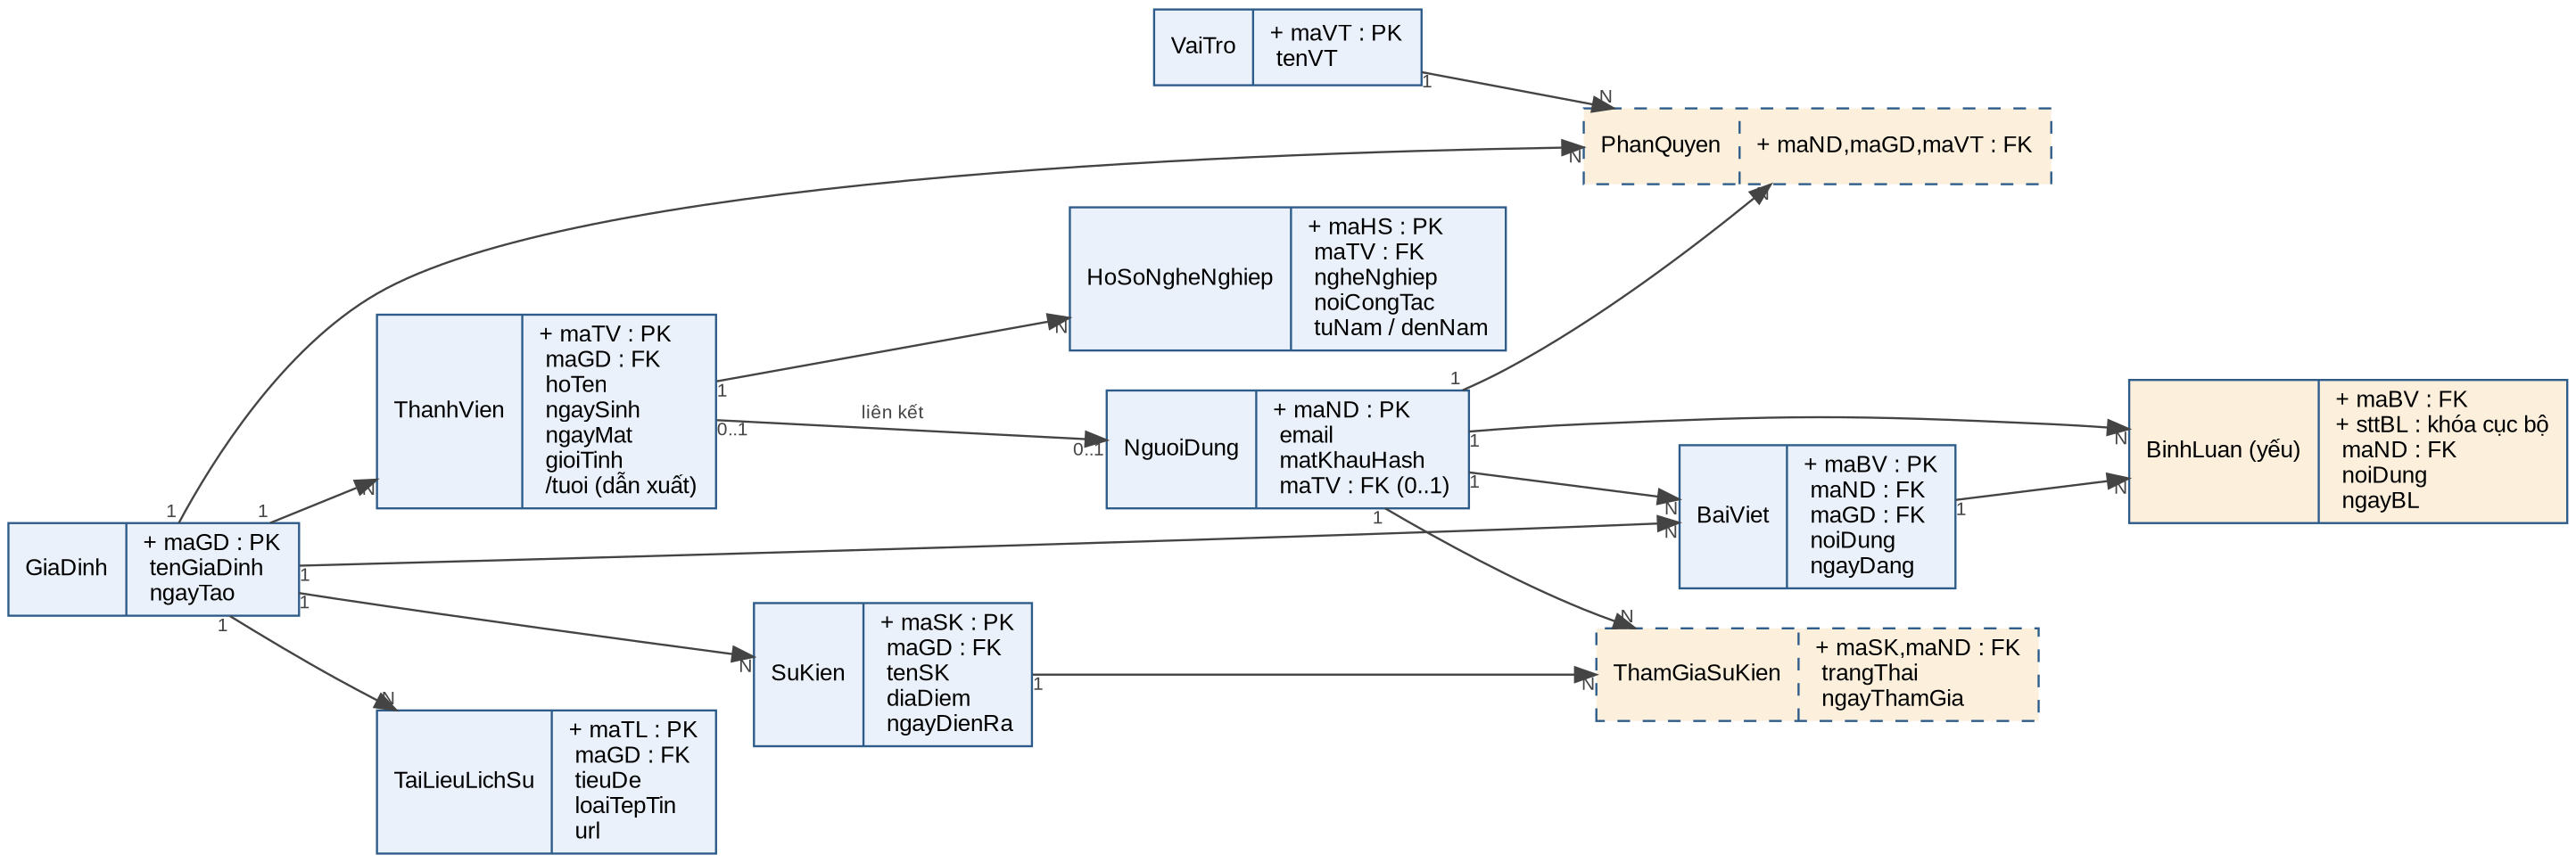
\includegraphics[width=0.95\linewidth]{images/erd_tongthe.png}
\caption{ERD tổng thể (ký pháp lớp UML: khối trên là thực thể, khối viền đứt là mối kết hợp có thuộc tính riêng)}
\end{figure}

\subsection*{Chi tiết mối kết hợp tự thân trên ThanhVien}
\addcontentsline{toc}{subsection}{Chi tiết mối kết hợp tự thân trên ThanhVien}

Vì quan hệ huyết thống và hôn nhân đều diễn ra giữa hai thể hiện của cùng một thực thể ThanhVien, cần tách rõ thành hai mối kết hợp độc lập để tránh nhầm lẫn khi chuyển sang lược đồ quan hệ:

\begin{figure}[htbp]
\centering
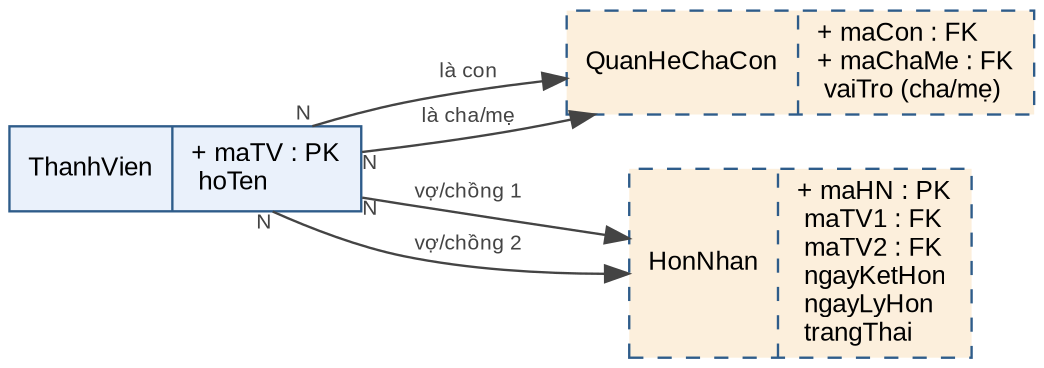
\includegraphics[width=0.75\linewidth]{images/erd_tuthanpk.png}
\caption{Mối kết hợp tự thân: QuanHeChaCon và HonNhan trên thực thể ThanhVien}
\end{figure}

\section{Đặc tả EER --- Chuyên biệt hóa tài khoản}

Hệ thống phân biệt hai dạng tài khoản theo mức quyền: Quản trị gia đình (được tạo/sửa cấu trúc gia phả) và Thành viên thường (chỉ xem/tương tác). Áp dụng chuyên biệt hóa \{disjoint, complete\}:

Ánh xạ chuyên biệt hóa này được đưa chính thức vào lược đồ quan hệ ở mục 4.1 (hai bảng QuanTriGiaDinh, ThanhVienThuong), thay vì chỉ dừng ở mức khái niệm.

\begin{infobox}
\begin{verbatim}
NguoiDung(maND, email, matKhauHash)
 +-- QuanTriGiaDinh(maND PK/FK, quyenDacBiet)
 `-- ThanhVienThuong(maND PK/FK)
\end{verbatim}
\end{infobox}

\section{Kiểm chứng bằng dữ liệu mẫu}

\begin{itemize}
  \item Thêm một ThanhVien chưa có tài khoản NguoiDung (thành viên đã mất, thế hệ trước) → mô hình vẫn hợp lệ nhờ bản số 0..1.
  \item Thêm một ThanhVien có 2 lần HonNhan tại hai thời điểm khác nhau → hợp lệ nhờ HonNhan là association class riêng, không gộp vào ThanhVien.
  \item Xóa một GiaDinh → cần xác định chính sách xóa (cascade hoặc chặn) cho ThanhVien, BaiViet, SuKien liên quan --- ghi chú này chuyển thành ràng buộc ON DELETE ở Chương 5.
\end{itemize}


\chapter{THIẾT KẾ LOGIC}

\section{Ánh xạ ERD sang lược đồ quan hệ}

Áp dụng quy tắc ánh xạ chuẩn: thực thể mạnh → một quan hệ; mối kết hợp 1:N → khóa chính phía 1 đưa sang phía N làm khóa ngoại; mối kết hợp M:N → tạo quan hệ trung gian với khóa chính là tổ hợp hai khóa ngoại; thực thể yếu → khóa chính là khóa chủ ghép khóa cục bộ.

\begin{infobox}
\footnotesize
\begin{verbatim}
NguoiDung(maND, email, matKhauHash, maTV FK, ngayTao)
GiaDinh(maGD, tenGiaDinh, ngayTao)
ThanhVien(maTV, maGD FK, hoTen, ngaySinh, ngayMat, gioiTinh)
QuanHeChaCon(maCon FK, maChaMe FK, vaiTro) -- PK: (maCon, maChaMe)
HonNhan(maHN, maTV1 FK, maTV2 FK, ngayKetHon, ngayLyHon, trangThai)
VaiTro(maVT, tenVT)
PhanQuyen(maND FK, maGD FK, maVT FK) -- PK tổ hợp 3 khóa
BaiViet(maBV, maND FK, maGD FK, noiDung, ngayDang)
BinhLuan(maBV FK, sttBL, maND FK, noiDung, ngayBL) -- khóa: (maBV, sttBL)
SuKien(maSK, maGD FK, tenSK, diaDiem, ngayDienRa)
ThamGiaSuKien(maSK FK, maND FK, trangThai, ngayThamGia) -- PK: (maSK, maND)
HoSoNgheNghiep(maHS, maTV FK, ngheNghiep, noiCongTac, tuNam, denNam)
TaiLieuLichSu(maTL, maGD FK, tieuDe, loaiTepTin, url)
QuanTriGiaDinh(maND PK/FK, quyenDacBiet) -- ánh xạ chuyên biệt hóa 3.4,
                                            1:1 với NguoiDung
ThanhVienThuong(maND PK/FK) -- ánh xạ chuyên biệt hóa 3.4
NhatKyKiemToan(maNK, maND FK NULL, hanhDong, doiTuong, thoiGian)
\end{verbatim}
\end{infobox}

\section{Xác định phụ thuộc hàm (FD)}

Phụ thuộc hàm được rút ra trực tiếp từ quy tắc nghiệp vụ ở mục 2.2, làm cơ sở để kiểm tra và chứng minh chuẩn hóa:

\begin{infobox}
\begin{verbatim}
maTV -> maGD, hoTen, ngaySinh, ngayMat, gioiTinh
maND -> email, matKhauHash, maTV
(maCon, maChaMe) -> vaiTro
(maSK, maND) -> trangThai, ngayThamGia
maHS -> maTV, ngheNghiep, noiCongTac, tuNam, denNam
maBV -> maND, maGD, noiDung, ngayDang
(maBV, sttBL) -> maND, noiDung, ngayBL
maHN -> maTV1, maTV2, ngayKetHon, ngayLyHon, trangThai
maVT -> tenVT
maTL -> maGD, tieuDe, loaiTepTin, url
maNK -> maND, hanhDong, doiTuong, thoiGian
\end{verbatim}
\end{infobox}

\section{Kiểm tra và chứng minh chuẩn hóa}

\subsection{Dạng chuẩn 1 (1NF)}

Không có thuộc tính đa trị được lưu chung trong một cột. Ví dụ, số điện thoại liên hệ của ThanhVien nếu có nhiều giá trị sẽ được tách thành bảng riêng:

\begin{infobox}
\begin{verbatim}
LienHeThanhVien(maTV FK, loaiLienHe, giaTri)
  -- PK: (maTV, loaiLienHe, giaTri)
\end{verbatim}
\end{infobox}

\subsection{Dạng chuẩn 2 (2NF)}

Xét các quan hệ có khóa tổ hợp: ThamGiaSuKien(maSK, maND) → trangThai, ngayThamGia; QuanHeChaCon(maCon, maChaMe) → vaiTro; PhanQuyen(maND, maGD, maVT). Mọi thuộc tính không khóa đều phụ thuộc đầy đủ vào toàn bộ khóa tổ hợp, không có thuộc tính nào chỉ phụ thuộc một phần khóa → các quan hệ đạt 2NF.

Các quan hệ đơn khóa bổ sung ở 4.2 (HonNhan, VaiTro, TaiLieuLichSu, NhatKyKiemToan, QuanTriGiaDinh, ThanhVienThuong) đạt 2NF hiển nhiên vì khóa chính không phải tổ hợp. Riêng PhanQuyen không có thuộc tính không khóa nào nên điều kiện 2NF cũng thỏa mãn một cách hiển nhiên (không có gì để kiểm tra phụ thuộc bộ phận).

\subsection{Dạng chuẩn 3 (3NF) --- chứng minh bằng phản ví dụ}

Giả sử ban đầu gộp ThanhVien và GiaDinh thành một bảng ThanhVien\_GD(maTV, hoTen, maGD, tenGiaDinh). Khi đó tồn tại phụ thuộc bắc cầu:

\begin{center}
maTV → maGD, \quad maGD → tenGiaDinh \quad $\Rightarrow$ \quad maTV → tenGiaDinh \ (bắc cầu)
\end{center}

Điều này gây dị thường: đổi tên một GiaDinh phải sửa trên mọi dòng ThanhVien thuộc gia đình đó (bất thường sửa), và không thể tạo một GiaDinh mới nếu chưa có ThanhVien nào (bất thường thêm). Phân rã tách GiaDinh thành quan hệ riêng như ở mục 4.1 loại bỏ phụ thuộc bắc cầu này → đạt 3NF.

\subsection{Dạng chuẩn Boyce--Codd (BCNF)}

Với mọi FD không tầm thường X → Y trong các quan hệ đã liệt kê, vế trái X đều là siêu khóa (khóa chính hoặc khóa chính tổ hợp) của quan hệ tương ứng. Do đó toàn bộ lược đồ ở mục 4.1 đạt BCNF; không phát sinh phụ thuộc bất thường ngoài khóa.

Kết luận này nay bao quát toàn bộ các quan hệ đã liệt kê ở 4.1, kể cả các bảng bổ sung HonNhan, VaiTro, TaiLieuLichSu, NhatKyKiemToan, QuanTriGiaDinh và ThanhVienThuong --- tất cả đều có khóa chính là khóa đơn hoặc khóa ngoại 1:1, nên mọi FD không tầm thường đều xuất phát từ siêu khóa.

\section{Kiểm tra tính bảo toàn của phép phân rã}

Áp dụng điều kiện đủ (R1 $\cap$ R2) → R1 hoặc (R1 $\cap$ R2) → R2: ví dụ ThanhVien và GiaDinh giao nhau ở maGD, là khóa chính của GiaDinh → phép phân rã bảo toàn kết nối. Tương tự, BaiViet và BinhLuan giao nhau ở maBV, là khóa chính của BaiViet → bảo toàn kết nối, không sinh dòng giả khi JOIN lại.


\chapter{THIẾT KẾ VẬT LÝ}

\section{Đặc tả workload dự kiến}

Thiết kế vật lý bắt đầu từ câu hỏi: truy vấn nào lặp lại đủ nhiều để đáng trả chi phí lưu trữ và bảo trì chỉ mục?

\begin{center}
\begin{tabularx}{\linewidth}{@{}>{\raggedright\arraybackslash}p{4.3cm}l>{\raggedright\arraybackslash}X@{}}
\toprule
\textbf{Truy vấn} & \textbf{Tần suất} & \textbf{Quyết định vật lý} \\
\midrule
Tra cứu ThanhVien theo maTV & Rất cao & Clustered index (khóa chính) \\
Liệt kê ThanhVien theo maGD & Cao & Chỉ mục phụ trên ThanhVien.maGD \\
Truy vấn cây gia phả (đệ quy cha--con) & Cao & Chỉ mục hai chiều trên QuanHeChaCon(maChaMe, maCon) và (maCon, maChaMe) \\
Feed bài viết theo GiaDinh, mới nhất trước & Cao & Chỉ mục kết hợp BaiViet(maGD, ngayDang DESC) \\
RSVP sự kiện theo SuKien & Trung bình & Chỉ mục trên ThamGiaSuKien(maSK) \\
Semantic search AI & Trung bình & Vector/full-text index riêng --- ngoài phạm vi B+ tree quan hệ, xem mục 5.5 \\
Thống kê dashboard theo GiaDinh & Thấp & Không cần chỉ mục riêng, dùng truy vấn tổng hợp \\
\bottomrule
\end{tabularx}
\end{center}

\section{Kịch bản DDL (SQL Server)}

\begin{sqlcode}
\begin{verbatim}
CREATE TABLE GiaDinh (
  maGD varchar(20) NOT NULL PRIMARY KEY,
  tenGiaDinh nvarchar(200) NOT NULL,
  ngayTao datetime2 NOT NULL DEFAULT SYSDATETIME()
);

CREATE TABLE ThanhVien (
  maTV varchar(20) NOT NULL PRIMARY KEY,
  maGD varchar(20) NOT NULL,
  hoTen nvarchar(150) NOT NULL,
  ngaySinh date NULL,
  ngayMat date NULL,
  gioiTinh varchar(10) NULL,
  CONSTRAINT FK_TV_GD FOREIGN KEY (maGD) REFERENCES GiaDinh(maGD)
    ON DELETE CASCADE
);

CREATE TABLE QuanHeChaCon (
  maCon varchar(20) NOT NULL,
  maChaMe varchar(20) NOT NULL,
  vaiTro varchar(10) NOT NULL,
  CONSTRAINT PK_QHCC PRIMARY KEY (maCon, maChaMe),
  CONSTRAINT FK_QHCC_Con FOREIGN KEY (maCon) REFERENCES ThanhVien(maTV)
    ON DELETE CASCADE,
  CONSTRAINT FK_QHCC_Cha FOREIGN KEY (maChaMe) REFERENCES ThanhVien(maTV)
    ON DELETE NO ACTION
);

CREATE TABLE NguoiDung (
  maND varchar(20) NOT NULL PRIMARY KEY,
  email nvarchar(150) NOT NULL UNIQUE,
  matKhauHash varchar(255) NOT NULL,
  maTV varchar(20) NULL UNIQUE,
  ngayTao datetime2 NOT NULL DEFAULT SYSDATETIME(),
  CONSTRAINT FK_ND_TV FOREIGN KEY (maTV) REFERENCES ThanhVien(maTV)
    ON DELETE SET NULL
);

CREATE TABLE BaiViet (
  maBV varchar(20) NOT NULL PRIMARY KEY,
  maND varchar(20) NOT NULL,
  maGD varchar(20) NOT NULL,
  noiDung nvarchar(max) NOT NULL,
  ngayDang datetime2 NOT NULL DEFAULT SYSDATETIME(),
  CONSTRAINT FK_BV_ND FOREIGN KEY (maND) REFERENCES NguoiDung(maND)
    ON DELETE NO ACTION,
  CONSTRAINT FK_BV_GD FOREIGN KEY (maGD) REFERENCES GiaDinh(maGD)
    ON DELETE CASCADE
);

-- Luu y: FK_QHCC_Con va FK_QHCC_Cha cung tro ve ThanhVien; SQL Server
-- khong cho phep CASCADE tren ca hai duong vi gay "multiple cascade
-- paths". Chi dat CASCADE o chieu Con, chieu Cha dung NO ACTION va
-- don dep bang trigger/tang ung dung.

CREATE TABLE VaiTro (
  maVT varchar(20) NOT NULL PRIMARY KEY,
  tenVT nvarchar(100) NOT NULL
);

CREATE TABLE PhanQuyen (
  maND varchar(20) NOT NULL,
  maGD varchar(20) NOT NULL,
  maVT varchar(20) NOT NULL,
  CONSTRAINT PK_PhanQuyen PRIMARY KEY (maND, maGD, maVT),
  CONSTRAINT FK_PQ_ND FOREIGN KEY (maND) REFERENCES NguoiDung(maND)
    ON DELETE CASCADE,
  CONSTRAINT FK_PQ_GD FOREIGN KEY (maGD) REFERENCES GiaDinh(maGD)
    ON DELETE CASCADE,
  CONSTRAINT FK_PQ_VT FOREIGN KEY (maVT) REFERENCES VaiTro(maVT)
    ON DELETE CASCADE
);

CREATE TABLE HonNhan (
  maHN varchar(20) NOT NULL PRIMARY KEY,
  maTV1 varchar(20) NOT NULL,
  maTV2 varchar(20) NOT NULL,
  ngayKetHon date NOT NULL,
  ngayLyHon date NULL,
  trangThai varchar(20) NOT NULL,
  CONSTRAINT FK_HN_TV1 FOREIGN KEY (maTV1) REFERENCES ThanhVien(maTV)
    ON DELETE NO ACTION,
  CONSTRAINT FK_HN_TV2 FOREIGN KEY (maTV2) REFERENCES ThanhVien(maTV)
    ON DELETE NO ACTION
);

-- Rang buoc "khong chong lap thoi gian" giua cac lan HonNhan cua
-- cung mot ThanhVien (muc 6.2) can trigger, khong bieu dien duoc
-- bang CHECK/FK thuan tuy.

CREATE TABLE BinhLuan (
  maBV varchar(20) NOT NULL,
  sttBL int NOT NULL,
  maND varchar(20) NOT NULL,
  noiDung nvarchar(max) NOT NULL,
  ngayBL datetime2 NOT NULL DEFAULT SYSDATETIME(),
  CONSTRAINT PK_BinhLuan PRIMARY KEY (maBV, sttBL),
  CONSTRAINT FK_BL_BV FOREIGN KEY (maBV) REFERENCES BaiViet(maBV)
    ON DELETE CASCADE,
  CONSTRAINT FK_BL_ND FOREIGN KEY (maND) REFERENCES NguoiDung(maND)
    ON DELETE NO ACTION
);

CREATE TABLE SuKien (
  maSK varchar(20) NOT NULL PRIMARY KEY,
  maGD varchar(20) NOT NULL,
  tenSK nvarchar(200) NOT NULL,
  diaDiem nvarchar(200) NULL,
  ngayDienRa datetime2 NOT NULL,
  CONSTRAINT FK_SK_GD FOREIGN KEY (maGD) REFERENCES GiaDinh(maGD)
    ON DELETE CASCADE
);

CREATE TABLE ThamGiaSuKien (
  maSK varchar(20) NOT NULL,
  maND varchar(20) NOT NULL,
  trangThai varchar(20) NOT NULL,
  ngayThamGia datetime2 NOT NULL DEFAULT SYSDATETIME(),
  CONSTRAINT PK_TGSK PRIMARY KEY (maSK, maND),
  CONSTRAINT FK_TGSK_SK FOREIGN KEY (maSK) REFERENCES SuKien(maSK)
    ON DELETE CASCADE,
  CONSTRAINT FK_TGSK_ND FOREIGN KEY (maND) REFERENCES NguoiDung(maND)
    ON DELETE CASCADE
);

CREATE TABLE HoSoNgheNghiep (
  maHS varchar(20) NOT NULL PRIMARY KEY,
  maTV varchar(20) NOT NULL,
  ngheNghiep nvarchar(150) NOT NULL,
  noiCongTac nvarchar(200) NULL,
  tuNam int NOT NULL,
  denNam int NULL,
  CONSTRAINT FK_HS_TV FOREIGN KEY (maTV) REFERENCES ThanhVien(maTV)
    ON DELETE CASCADE
);

CREATE TABLE TaiLieuLichSu (
  maTL varchar(20) NOT NULL PRIMARY KEY,
  maGD varchar(20) NOT NULL,
  tieuDe nvarchar(200) NOT NULL,
  loaiTepTin varchar(20) NOT NULL,
  url nvarchar(400) NOT NULL,
  CONSTRAINT FK_TL_GD FOREIGN KEY (maGD) REFERENCES GiaDinh(maGD)
    ON DELETE CASCADE
);

CREATE TABLE NhatKyKiemToan (
  maNK bigint IDENTITY(1,1) NOT NULL PRIMARY KEY,
  maND varchar(20) NULL,
  hanhDong varchar(20) NOT NULL,
  doiTuong nvarchar(100) NOT NULL,
  thoiGian datetime2 NOT NULL DEFAULT SYSDATETIME(),
  CONSTRAINT FK_NK_ND FOREIGN KEY (maND) REFERENCES NguoiDung(maND)
    ON DELETE SET NULL
);

-- maND NULL cho phep log ton tai ke ca khi tai khoan nguoi thuc hien
-- da bi xoa.

CREATE TABLE QuanTriGiaDinh (
  maND varchar(20) NOT NULL PRIMARY KEY,
  quyenDacBiet nvarchar(200) NOT NULL,
  CONSTRAINT FK_QTGD_ND FOREIGN KEY (maND) REFERENCES NguoiDung(maND)
    ON DELETE CASCADE
);

CREATE TABLE ThanhVienThuong (
  maND varchar(20) NOT NULL PRIMARY KEY,
  CONSTRAINT FK_TVT_ND FOREIGN KEY (maND) REFERENCES NguoiDung(maND)
    ON DELETE CASCADE
);

-- Rang buoc {disjoint}: mot maND chi nen xuat hien o MOT trong hai
-- bang tren;
-- FK/PK thuan tuy chua chan duoc dieu nay, can CHECK constraint
-- kieu ung dung hoac trigger.
\end{verbatim}
\end{sqlcode}

\section{Khai báo chỉ mục theo workload}

\begin{sqlcode}
\begin{verbatim}
CREATE INDEX IX_TV_GiaDinh
  ON ThanhVien(maGD);

CREATE INDEX IX_QHCC_ChaMe_Con
  ON QuanHeChaCon(maChaMe, maCon);

CREATE INDEX IX_BaiViet_GiaDinh_Ngay
  ON BaiViet(maGD, ngayDang DESC);

CREATE INDEX IX_ThamGiaSuKien_SuKien
  ON ThamGiaSuKien(maSK);

-- Da bo IX_QHCC_Con_ChaMe: trung thu tu cot voi PRIMARY KEY (maCon,
-- maChaMe) da khai bao o 5.2 (mac dinh clustered trong SQL Server)
-- nen chi muc rieng la du thua.

CREATE INDEX IX_NhatKyKiemToan_ThoiGian
  ON NhatKyKiemToan(thoiGian);
\end{verbatim}
\end{sqlcode}

Lưu ý về độ chọn lọc (selectivity): cột gioiTinh hoặc trangThai (chỉ 2--3 giá trị phân biệt) không nên tạo chỉ mục B+ tree riêng vì mỗi giá trị trả về quá nhiều dòng, làm chỉ mục kém hiệu quả --- phù hợp nguyên tắc Algorithm 4.1 đã học.

\section{Phân vùng dữ liệu (Partitioning)}

Các bảng tăng trưởng nhanh nhưng ít truy vấn ngẫu nhiên như NhatKyKiemToan và log truy vấn AI nên được phân vùng theo thời gian để giảm kích thước chỉ mục hoạt động và hỗ trợ dọn dữ liệu cũ:

\begin{sqlcode}
\begin{verbatim}
CREATE PARTITION FUNCTION pf_Nam(int)
  AS RANGE LEFT FOR VALUES (2024, 2025, 2026);

CREATE PARTITION SCHEME ps_Nam
  AS PARTITION pf_Nam ALL TO ([PRIMARY]);
\end{verbatim}
\end{sqlcode}

\section{Hướng mở rộng vượt phạm vi B+ tree quan hệ}

\begin{itemize}
  \item Cây gia phả nhiều thế hệ: cân nhắc mô hình Closure Table hoặc Materialized Path bổ sung cho QuanHeChaCon để truy vấn tổ tiên/hậu duệ nhanh hơn CTE đệ quy thuần túy.
  \item Semantic search AI: cần chỉ mục vector (ví dụ trên nền tảng hỗ trợ vector search) song song với dữ liệu quan hệ, nằm ngoài phạm vi chỉ mục B+ tree/Hash truyền thống.
  \item Bảng nội dung lớn (BaiViet, TaiLieuLichSu) có thể cân nhắc columnstore index nếu phát sinh nhu cầu phân tích thống kê nội dung ở quy mô lớn.
\end{itemize}


\chapter{KẾT LUẬN}

\section{Kết quả đạt được}

\begin{itemize}
  \item Xây dựng được bộ quy tắc nghiệp vụ và danh sách thực thể bám sát chức năng thực tế của FamilyConnect.
  \item Thiết kế ERD/EER xử lý đúng điểm khó nhất của đề tài: mối kết hợp tự thân (huyết thống, hôn nhân) trên thực thể ThanhVien.
  \item Ánh xạ và chứng minh lược đồ quan hệ đạt 3NF/BCNF, loại bỏ các dị thường thêm/sửa/xóa điển hình.
  \item Đề xuất chỉ mục và phân vùng vật lý bám theo workload dự kiến của hệ thống, phù hợp SQL Server.
\end{itemize}

\section{Hạn chế và hướng phát triển}

\begin{itemize}
  \item Chưa mô hình hóa chi tiết ràng buộc thời gian không chồng lấp của HonNhan (cần trigger hoặc kiểm tra ở tầng ứng dụng).
  \item Chưa đi sâu thiết kế hạ tầng lưu trữ vector cho các dịch vụ AI (semantic search, gợi ý).
  \item Có thể mở rộng mô hình Closure Table cho cây gia phả khi số thế hệ và khối lượng truy vấn tăng cao.
  \item Ràng buộc "tối đa hai cha/mẹ trực tiếp" (2.2) và ràng buộc \{disjoint\} giữa QuanTriGiaDinh/ThanhVienThuong (3.4) chưa thể biểu diễn thuần bằng khóa chính/khóa ngoại --- cần CHECK constraint kiểu ứng dụng hoặc trigger, hiện chưa hiện thực trong phạm vi đề án.
  \item CamXuc (2.1) tạm loại khỏi phạm vi thiết kế bản này; có thể bổ sung như một thực thể yếu tương tự BinhLuan ở hướng phát triển tiếp theo.
\end{itemize}


\chapter*{Tài liệu tham khảo}
\addcontentsline{toc}{chapter}{Tài liệu tham khảo}

\begin{itemize}
  \item Bài giảng Thiết kế Cơ sở dữ liệu --- Chương 1--4, Nguyen Van Chien, Trường Đại học Giao thông Vận tải, 2026.
  \item Đặc tả đề tài FamilyConnect: AI-powered Digital Family Community Platform.
\end{itemize}



\end{document}

